\documentclass[preprint]{aastex} 

\usepackage[top=1in, bottom=1in, left=1in, right=1in]{geometry}
\usepackage{amsmath}
\usepackage{graphicx}
\usepackage{mdwlist}
\usepackage{natbib}
\usepackage{natbibspacing}
\setlength{\bibspacing}{0pt}
\setlength{\parskip}{0pt}
\setlength{\parsep}{0pt}
\setlength{\headsep}{0pt}  
\setlength{\topskip}{0pt}
\setlength{\topmargin}{0pt}
\setlength{\topsep}{0pt}
\setlength{\partopsep}{0pt}
\setlength{\footnotesep}{8pt}
\pagestyle{empty}
\citestyle{aa}

\def\kperp{k_{\bot}}
\def\kpar{k_{\|}}
\def\k{{\bf k}}
\def\sky{{\theta}}
\def\HI{{H{\small I }}}

%\usepackage{subfig}
%\usepackage[countmax]{subfloat}

%Project Description (8-pages maximum), including the following:
%- A statement of which of the four categories of MSIP is most appropriate
%for this proposal as the first sentence (see section II. Program Description).
%- A scientific justification. For Open Access Capabilities, explain the
%uniqueness and lack of general availability of the capability.
%- A description of the broader impacts, including student training.
%- A description of benefits to the community (observing time, data products, etc.)
%- An outline of the project management plan (where appropriate).
%Note: Results from Prior NSF Support should not be included. Links to URLs may
%not be used.
\begin{document}
%\title{Hydrogen Epoch of Reionization Array}
\title{HERA: Illuminating Our Early Universe\\
{\it For the Mid-Scale Science Projects category of the Mid-Scale Innovations Program}} 

% A statement of which of the four categories of MSIP is most appropriate
%for this proposal as the first sentence (see section II. Program Description).

%This proposal targets the Mid-Scale Science Projects category of the Mid-Scale Innovations Program solicitation. The Hydrogen Epoch of Reionization Arrays (HERA) is a program for using the unique capabilities of the 21~cm hyperfine line to trace neutral hydrogen through the cosmic dawn of our Universe.  The HERA roadmap that was submitted to the {\it New Worlds, New Horizons of Astronomy and Astrophysics} 2010 decadal survey, (hereafter NWNH) was given ``top priority in this [Radio, Millimeter, and Sub-millimeter] category of recommended new facilities for mid-scale funding." The HERA roadmap proceeded in three stages: HERA-IB called for \$25M to complete the PAPER and MWA experiments; HERA-II budgeted \$62M for an array with 0.1 km$^2$ of collecting area capable of characterizing the power spectrum of cosmic reionization in detail; HERA-III targeted 1 km$^2$ of collecting area to image reionization structures in detail.

{ \setlength{\parindent}{0cm}
%The major stages in the history of our Universe are written in the phases of
%hydrogen.
The Hydrogen Epoch of Reionization Arrays (HERA) roadmap is a staged
program that uses the unique properties of the 21~cm line from neutral
hydrogren to probe the evolution of the intergalactic medium (IGM) during the
Epoch of Reionization (EoR) and the preceding Dark Ages. Cosmic reionization
corresponds to the epoch when the first stars and black holes reionize the
neutral IGM that pervaded the Universe following cosmic recombination, roughly
0.5~Gyr to 1~Gyr after the Big Bang. Direct observation of the evolution of
large scale structure via the \HI 21~cm line will have a profound impact on our
understanding of the birth of the first galaxies and black holes, their
influence on the IGM, and cosmology.}  

HERA was given the ``top priority in the Radio, Millimeter, and Sub-millimeter
category of recommended new facilities for mid-scale funding" as part of the
{\it New Worlds, New Horizons of Astronomy and Astrophysics} decadal survey,
(\citealt{astro2010}; hereafter NWNH).  
% XXX some of this conflicts/repeats with the next paragraph
The HERA roadmap envisioned a series of
radio interferometers constructed throughout the decade, starting with the
PAPER and MWA instruments (Donald C. Backer Precision Array for Probing the
Epoch of Reionization; Murchison Widefield Array) aimed at characterizing
foregrounds and a first effort to detect the EoR power
spectrum, a second-generation instrument to measure the EoR power spectrum in
detail and reveal how early structure in the universe formed, and a
third-generation instrument late in the decade to image the EoR. 

Using the advances spearheaded by 
first-generation HERA instruments --- the Donald C. Backer Precision
Array for Probing the Epoch of Reionization (PAPER) and the Murchison Widefield Array (MWA) ---
we propose a staged
build-out of HERA
through arrays of 127, 331, and 568 elements, 
observing in the 50--225MHz band, 
with each stage improving our 
understanding of the HI 21cm signal from reionization.
Taken together, this program 
not only fulfills the goal of detailed power spectrum
characterization as a second-generation HERA experiment, but also is
capable of imaging the EoR, a task previously considered possible only for
third-generation instruments.

% XXX Are we ok without a document map?

\vspace{-0.25in}
\section{Scientific Justification}
\label{SJsec}

The last unexplored phase in the evolution of luminous structures in the
Universe begins with the birth of the first stars and culminates with the full
ionization of the IGM $\sim$500 Myrs later.  Whether during the Dark Ages
(z$\ge$15) or the Epoch of Reionization (z$\sim$15--6), a wealth of
astrophysical and cosmological phenomena are at play.  The precise properties
of the IGM depend on the nature and distribution of the first luminous sources
(eg. typical masses, UV escape fractions, biased structure formation), the
efficiency and abundance of heating sources (eg.  X-ray binaries, shocks, or
even dark matter annihilations), the formation of the first supermassive black
holes, and the relative velocity of baryonic matter and dark-matter halos,
among other effects.  Exploration of the Dark Ages and EoR and the evolution of
the IGM during these epochs has been called out as one of the top three
``priority science objectives chosen by the [NWNH] survey committee for the
decade 2012-2021."

Thus far, a number of indirect probes have been used to understand cosmic
reionization.  These include observations of Gunn-Peterson attenuation by the
IGM toward the most distant quasars \citep{fan_et_al2006},
kinetic Sunyaev-Zel'dovich features in the CMB \citep{zahn_et_al2012}, CMB
anisotropy and polarization \citep{page_et_al2007,planck_et_al2013}, and the
demographics of Ly$\alpha$ emitting galaxies
\citep{treu_et_al2013}, as summarized in Figure~\ref{fig:x_i_Xray}a.  Unfortunately,
these ground-breaking results have limited reach: the
Gunn-Peterson effect and related phenomena saturate at low neutral fractions,
and the CMB provides only an integral measure of the optical depth
back to recombination.  Moreover, many of these indirect observations are in
tension with one another, underscoring both the difficulty in interpreting
their results and the fact that reionization was a complex process.


\begin{figure}[t]\centering
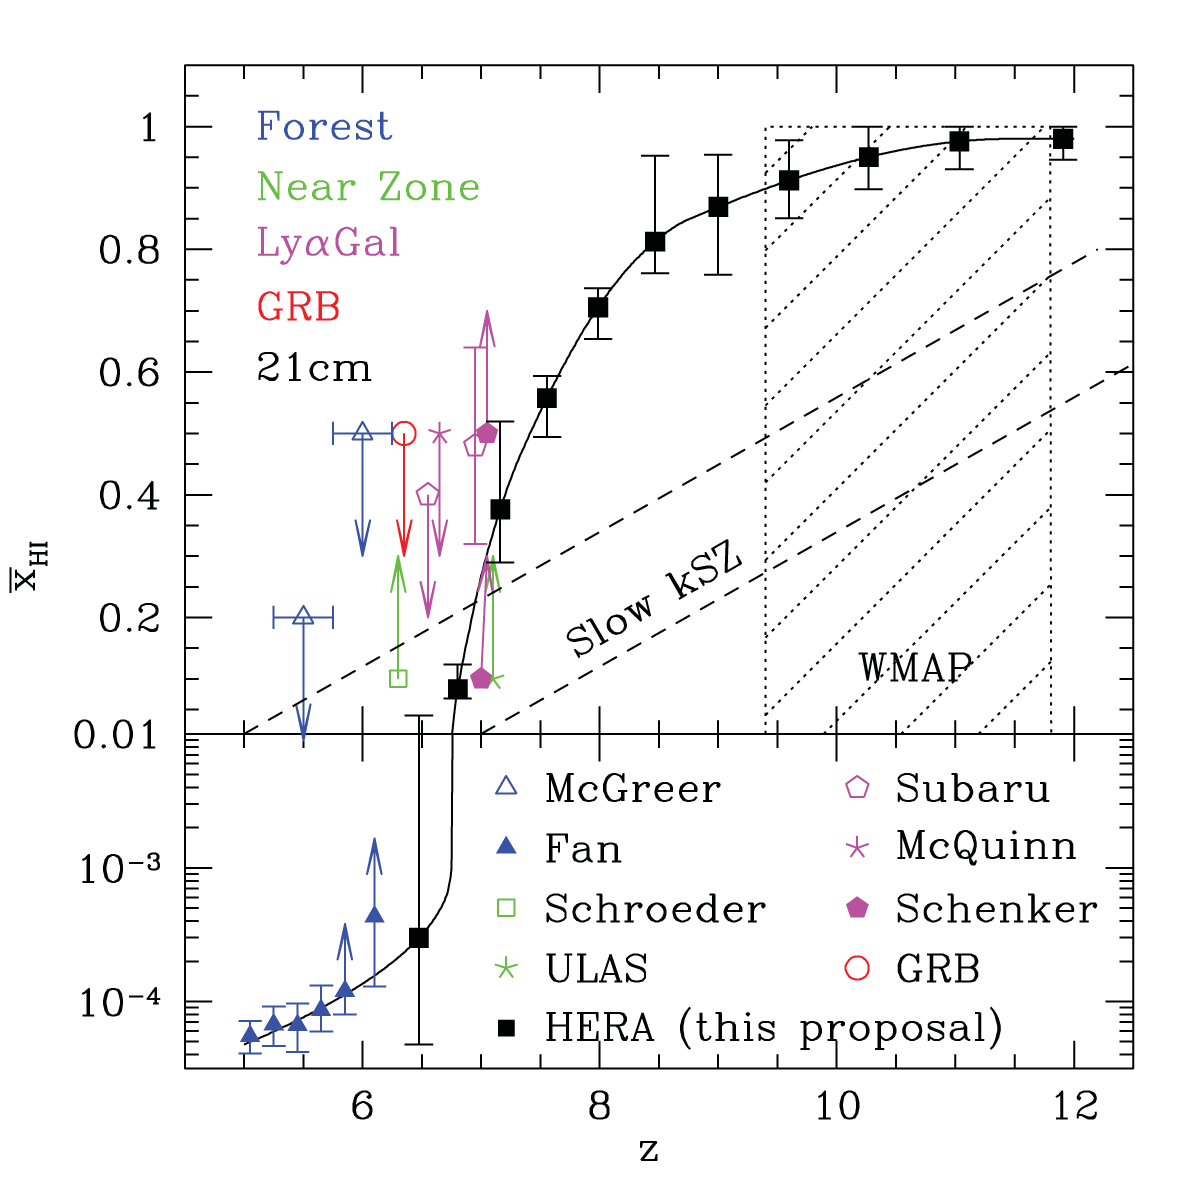
\includegraphics[height=2.25in]{plots/constraints.pdf} ~ % gap
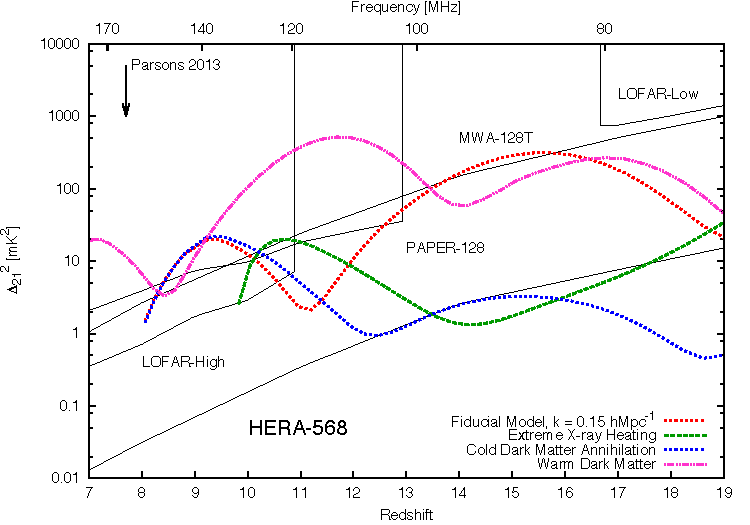
\includegraphics[height=2.25in]{plots/Xray.pdf} \caption{\small Left: A
theoretical reionization model, overlaid with current constraints
\citep{robertson_2013}, as well as the predicted constraints from HERA~568. %
XXX or is it HERA~331?  By adopting a fiducial model, measurements of the 21~cm
power spectrum (see Figure \ref{fig:eor_pspec}) determine the neutral fraction,
$x_{\rm\HI}$, of the universe as a function of redshift.  At high redshifts,
21~cm emission may be the only probe of $x_{\rm\HI}$.
%Left: A theoretical model from \citet{robertson_2013} that fits the existing
%constraints for reionization. Existing measurements and limits are indicated,
%along with the simulated measurements HERA would provide by constraining the
%rise and fall of the 21~cm power spectrum (see Figure \ref{fig:eor_pspec}).
%[XXX: Update this plot when the Aaron/Josh comparison is done.] 
Right: HERA's substantial sensitivity at low frequencies opens a window to
pre-reionization physics.  Shown here are power spectrum amplitudes at
$k=0.15h\ {\rm Mpc}^{-1}$ as a function of redshift for various IGM heating
models, along with predicted sensitivities.  HERA has the potential to
transform our understanding of the physical processes at play in the early
universe by distunguishing between these scenarios.
%Right: HERA's ability to observe at relatively high sensitivity even at low
%frequencies opens a window to higher redshift pre-reionization physics.  Shown
%here is the amplitude of the power spectrum as a function of redshift (at $k =
%0.15$~hMpc$^{-1}$) for a variety of theoretical models with different IGM
%heating mechanisms.
}\label{fig:x_i_Xray} \end{figure}
% XXX comments from Carilli:
%2. fig 1a.  excellent. really excellent.  except i am not sure replicating the
%X axis ticks in the middle is the best way to go. perhaps just a dash line or
%something. the caption should point out that at this line it switches from log
%to linear Y scale. also, the  'slow kZ' lines are confusing. what do they
%mean?  if they really delimit some range in f(HI), then doesn't that violate
%our predictions?   i would just remove, since these limits were more
%aspirational than meaningful in the publication.


% XXX comments from Aguirre:
%I'm confused why the the section "The HERA program follows a staged buildout
%..." and its bullet points comes in the middle of the science justification.
%The next paragraph then returns to stating why 21 cm is important, and ends
%with a discussion of complex effects and modeling.  I'm not sure that those
%bullet points belong in this section at all, but if so, they should be at the
%end.  You've set up all the interesting science: now bang off how HERA is
%going to address it.  But some of this is redundant with what's in Section 3
%in terms of the phasing.
The 21~cm hyperfine transition has been recognized as potentially the most
powerful probe of the evolution of the IGM during cosmic reionization, and into
the preceding Dark Ages \citep{morales_wyithe2010,furlanetto_et_al2006}.  The
HERA program follows a staged buildout, starting with a 37 antenna prototype
followed by annual upgrades to 127, 331, and 568 antennas to unlock additional
scientific capability (see project description in \S \ref{PDsec}, and power
spectrum sensitivity Figure \ref{fig:eor_pspec}a).  This program 
provides powerful new capabilities for placing observational constraints
on reionization, and potentially on large scale structure
evolution during the dark ages.
Over the timeline of the project, this staged build-out enables the following science program:
% XXX awkward transition
%\begin{itemize}\setlength{\parskip}{0pt}\itemsep0pt
%\item {\bf Years 1 \& 2:} Perform deep continuum survey using HERA-37 in the target reionization fields for bright source characterization. 
%\item {\bf Year 3:} Hera~127 will have sufficient sensitivity to determine of the evolution of the reionization power spectrum. The results will determine the primary epoch of cosmic reionization (the `50\% neutral fraction zone'), and the length of time during which reionization `bubbles' dominated the HI power spectrum. These data will also place strong constraints on warming of the neutral IGM by X-rays, and hence the rate and density of black hole formation in the
%early universe (\citealt{pritchard_loeb2010}; see Figure \ref{fig:x_i_Xray}, left panel). Note that study of the neutral IGM during the key redshift range from $z$ = 8 to 10 is difficult using standard techniques based on eg.\ Ly$\alpha$ spectra or galaxy populations due to saturation of the Ly$\alpha$ attenuation. HERA is uniquely suited to probe this redshift gap (see Figure \ref{fig:x_i_Xray}, right panel). 
%\item {\bf Year 4:} HERA~331 will make high sensitivity power spectral measurements over a significant range in wavenumber. The detailed shape of the power spectrum will be measured, dictating the nature and distribution of the first galaxies that dominate cosmic  reionization. Is early galaxy formation highly biased, or more uniformly distributed (inside-out vs.\ outside-in reionization)? Is reionization dominated by low or high mass galaxies? What is the escape fraction of UV photons in early galaxies? How does feedback from early star formation affect low-mass galaxies? [former might be overstating things?] The change in the slope of the power spectrum of 21~cm emission through reionization (Figure \ref{fig:eor_pspec}) determines the size of ionization bubbles at various stages of reionization, which constrains the relative contributions to the ionizing background of halos as a function of mass, and helps us understand how efficiently early structures cooled and formed stars. This array will also provide the first images of the largest scale structures during reionization, and determine how velocity streaming between baryonic  matter and the dark matter halos affected early structure formation and the onset of Ly$\alpha$ emission \citep{visbal_et_al2012}.
%\item {\bf Year 5:} HERA 568 will be a powerful instrument to characterized the power-spectrum through the reionization into the dark ages, as well as for direct imaging of the IGM during reionization. Imaging will be particularly important for comparison with large scale galaxy surveys that extended into cosmic reionization (see section ?? below). HERA-568 will have the sensitivity to push toward higher redshifts (lower frequencies), into the cosmic dark ages. More on Xray heating and dark matter annihiliation dark ages here...
%\end{itemize}

\begin{itemize}\setlength{\parskip}{0pt}\itemsep0pt
% XXX comments from Liu: On a quick skim, it's not hard to imagine that a
% reviewer might look at the first list and assume that we're jumping right to
% HERA 127.  I know it does say in the text that we'll be "starting with a 37
% antenna prototype", but it's kinda buried.  I think it would help a little
% bit if we omitted the "FY XXXX" labels in the first bulleted list.  That
% seems more appropriate for the second list, and by starting the first list
% with a date, it sounds like nothing interesting will happen before then.
% Also, are we going to make the case that if, as expected, the first
% generation fails to make a detection because reionization isn't surprisingly
% bright, that HERA 37 will do it? (I'm talking about just a single positive
% detection, rather than constraining the timing and duration, which we say
% HERA 127 will do).

\item {\bf FY 2017} HERA~127 will measure the rise and fall of the EoR power
spectrum, constraining the timing and duration of reionization.

\item {\bf FY 2018} HERA~331 will measure the shape of the power spectrum over
a significant range in wavenumber, determining the features and distribution of
the first galaxies that dominate cosmic reionization.
Figure~\ref{fig:x_i_Xray}a shows the direct constraints on reionization
HERA~331 will be able to provide.

%Is early galaxy formation highly biased, or more uniformly distributed (inside-out vs.\ outside-in reionization)? is reionization dominated by low or high mass galaxies? what is the escape fraction of UV photons in early galaxies? and how does feedback from early star formation affect low-mass galaxies? will all be determined by HERA~331.

\item {\bf FY 2019} HERA~568 will extend precision power-spectrum observations
into the dark ages and start direct imaging of the IGM during reionization.
Imaging will be particularly important for providing environmental context for
JWST observations and comparison with large scale galaxy surveys .
\end{itemize}

The study of the three-dimensional
evolution of large scale structure in the IGM via the \HI 21~cm line has the
potential to become `the richest of all cosmological data sets', and is expected
to have a science impact comparable to that of the CMB
\citep{barkana_loeb2005a,loeb_zaldarriaga2004}).  As emphasized in
NWNH: ``The panel concluded that to explore the discovery
area of the epoch of reionization, it is most important to develop new
capabilities to observe redshifted 21~cm \HI emission, building on the legacy of
current projects and increasing sensitivity and spatial resolution to
characterize the topology of the gas at reionization."  
%Although early 21~cm EoR experiments with limited sensitivity are targeting statistical detections
%of the power spectrum of reionization, the 21~cm signal versus redshift can
%eventually be reconstructed into three-dimensional maps of the evolution of
%cosmic structure that would greatly improve our understanding of the
%cosmological and astrophysical evolution of the universe
%\citep{furlanetto_et_al2006,mao_et_al2008,morales_wyithe2010}. 
As a high
sensitivity instrument with broad frequency coverage, HERA will be capable of
painting a consistent and uninterrupted picture of not just the EoR, but also
into the preceding Dark Ages.  

%%%

%The period beginning with the birth of the first luminous objects in the
%universe, and culminating with the ionization of the intergalactic medium (IGM)
%$\sim$500 Myrs later, is one of the last unexplored phases of cosmic evolution.
%The NWNH decadal survey highlighted the exploration of the epoch of reionization as %one of the three
%``priority science objectives chosen by the [NWNH] survey committee for the
%decade 2012-2021". Current observations of Gunn-Peterson absorption
%by the IGM toward the most distant quasars \citep{fan_et_al2006,bouwens_et_al2010}
%kinetic
%Sunyaev-Zel'dovich features in the CMB \citep{zahn_et_al2012}, and CMB
%anisotropy and polarization \citep{page_et_al2007,planck_et_al2013} are
%moderately in tension with one another, suggesting
%that reionization was a complex process.  Unfortunately, these ground-breaking %results are limited in
%diagnostic capabilities: the Gunn-Peterson effect saturates for even low
%neutral fractions, and the CMB provides only an integral measure of the
%Thompson optical depth back to recombination.
%
%Redshifted emission from the 21~cm hyperfine transition of neutral hydrogen has
%gained considerable attention as a unique tracer of the
%primordial IGM.  Directly observing the neutral IGM via this signal
%would be an achievement comparable with the discovery of the CMB.  As
%emphasized in NWNH: ``The panel concluded that to explore the
%discovery area of the epoch of reionization, it is most important to develop
%new capabilities to observe redshifted 21-cm \HI emission, building on the
%legacy of current projects and increasing sensitivity and spatial resolution to
%characterize the topology of the gas at reionization."
%Although early 21~cm EoR experiments with limited sensitivity are targeting
%statistical detections of the power spectrum of reionization, the 21~cm signal
%versus redshift and angle can eventually be reconstructed into
%three-dimensional maps of the evolution of cosmic structure that would greatly %improve
%our understanding of the cosmological
%and astrophysical evolution of the universe
%\citep{furlanetto_et_al2006,mao_et_al2008,morales_wyithe2010}.
%
%During the ``Dark Ages" (z$\sim$150--15) and cosmic reionization (z$\sim$15--6),
%21~cm emission is sensitive to a wealth of astrophysical and cosmological phenomena.

% XXX is there text from this paragraph to save?

%The new window into high-redshift 21~cm observations provided by HERA
%will begin to explore the rate and density of massive black holes formed in the
%early universe \citep{pritchard_loeb2010} via their X-ray emission (see Figure \ref{fig:Xray}), 
%how velocity streaming between baryonic 
%matter and the dark matter halos affected early structure formation and the onset
%of Ly$\alpha$ emission \citep{visbal_et_al2012}, and will lay the groundwork for future
%efforts to explore how 
%cosmological models can be improved via measurements of redshift-space distortions,
%artificial anisotropies introduced via the Alcock-Paczy\'inski effect, and
%gravitational lensing signals\citep{furlanetto_et_al2006}.
%As illustrated in Figure \ref{fig:x_i}, observing the 21~cm line 
%through this epoch with HERA-568 
%promises to determine the ionization history of our universe much more precisely,
%and at higher neutral fractions, than is possible with other existing techniques.  These measurements can
%be used to move beyond characterizing the timing and duration of reionization to
%explore which galaxies dominate the integrated UV luminosity density, what the escape fraction
%of UV photons is in early galaxies, and how feedback from early star formation affects low-mass galaxies and the integrated global %ionization profile versus
%redshift.  Moreover, measurements of the slope of the power spectrum of 21~cm emission through
%reionization (Figure \ref{fig:FourPanContour}) determine the size of ionization bubbles for at
%various stages of reionization, which
%constrains the relative contributions to the ionizing background of halos as a function of mass,
%and helps us understand how efficiently early structures cooled and formed stars.

%The evolution of the \HI 21~cm signal from the neutral IGM depends on miriad
%physical processes, including: general large scale structure evolution, IGM
%ionization by the first galaxies and black holes, and the complex interplay
%between the gas kinetic and excitation temperatures, and the temperature of the
%CMB \citep{furlanetto_et_al2006}. The gas kinetic temperature can be affected
%by shocks or pervasive X-rays from the first luminous sources, and the HI
%excitation temperature can be dictated by collisions, CMB photons, or resonant
%scattering of ambient Ly$\alpha$ photons, depending on epoch
%\citep{pritchard_loeb2012}.  The relative importance of these competing effects
%is sensitive to, among other things, the expansion of the universe, the
%ignition of the first stars and galaxies, the formation of the first massive
%black holes \citep{mesinger_et_al2013}, and the relative velocity of baryonic
%matter and dark-matter halos \citep{mcquinn_oleary2012}.  

In the past decade, considerable effort has gone into modeling the complex astrophysics
of reionization
\citep{santos_et_al2010,mesinger_et_al2011,wyithe_loeb2004}. However, bridging the
enormous scale difference between the self-shielding regions that are the
primary sinks of ionizing photons and volumes required for statistically
representative samples of cosmic structures remains an open problem.  
Basic constraints on theoretical models remain rudimentary, and the most
fundamental questions concerning the process of reionization remain open. 
When did
reionization occur, and over what timescale?  What objects dominated the
radiation field? how were the objects distributed? Did the first generation of
stars enhance or suppress the formation of subsequent stars in the original
halo and smaller nearby halos? Without measurements such as those made possible by HERA,
further progress on understanding first galaxy formation and
cosmic reionization remains problematic. 

%\begin{figure}[!ht]\centering
%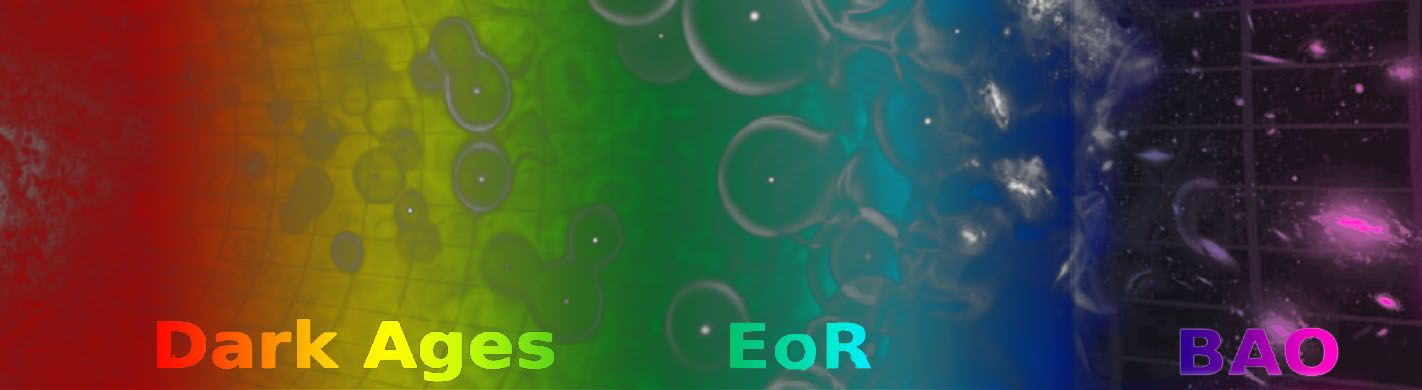
\includegraphics[width=6in]{plots/21cm_cosmo.jpg}
%\caption{\small
%The 21~cm hyperfine line of neutral hydrogen represents the next frontier in
%precision cosmology. Following recombination (left edge), the spin temperature
%of 21~cm emission is sensitive to the density and temperature of the
%intergalactic medium (IGM) through the Dark Ages, evolves with the heating and
%ionization of the IGM during the Epoch of Reionization (EoR), and
%traces the distribution of galaxies as the universe expands,
%leading up the the present day (right edge).  Color indicates
%redshift, which stretches the 21~cm line to frequencies ranging from 50 MHz
%(red) to 1.4 GHz (violet).
%}\label{fig:21cm_cosmo}
%\end{figure}

\begin{figure}[t]\centering 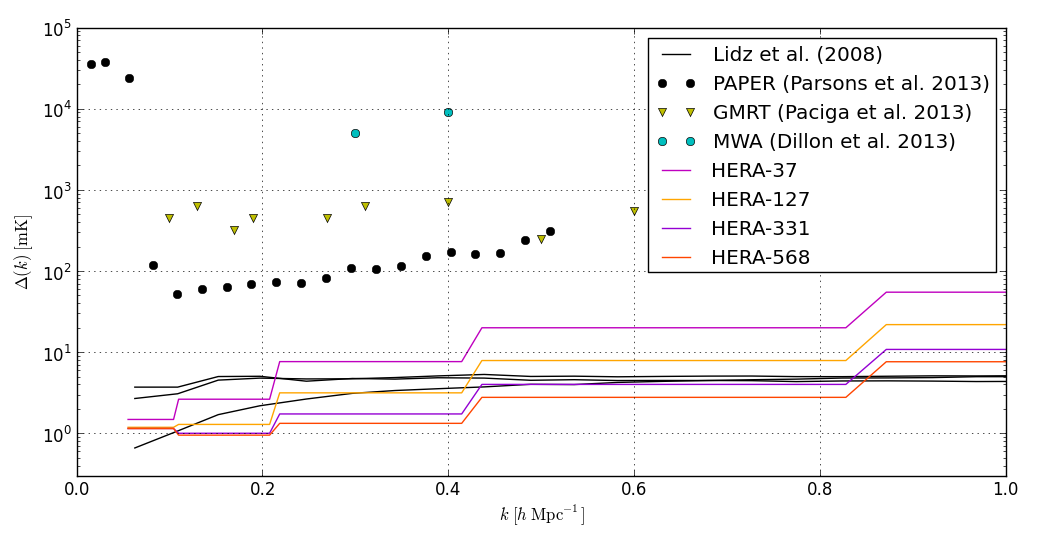
\includegraphics[height=2.20
in]{plots/eor_pspec.png} ~ % gap 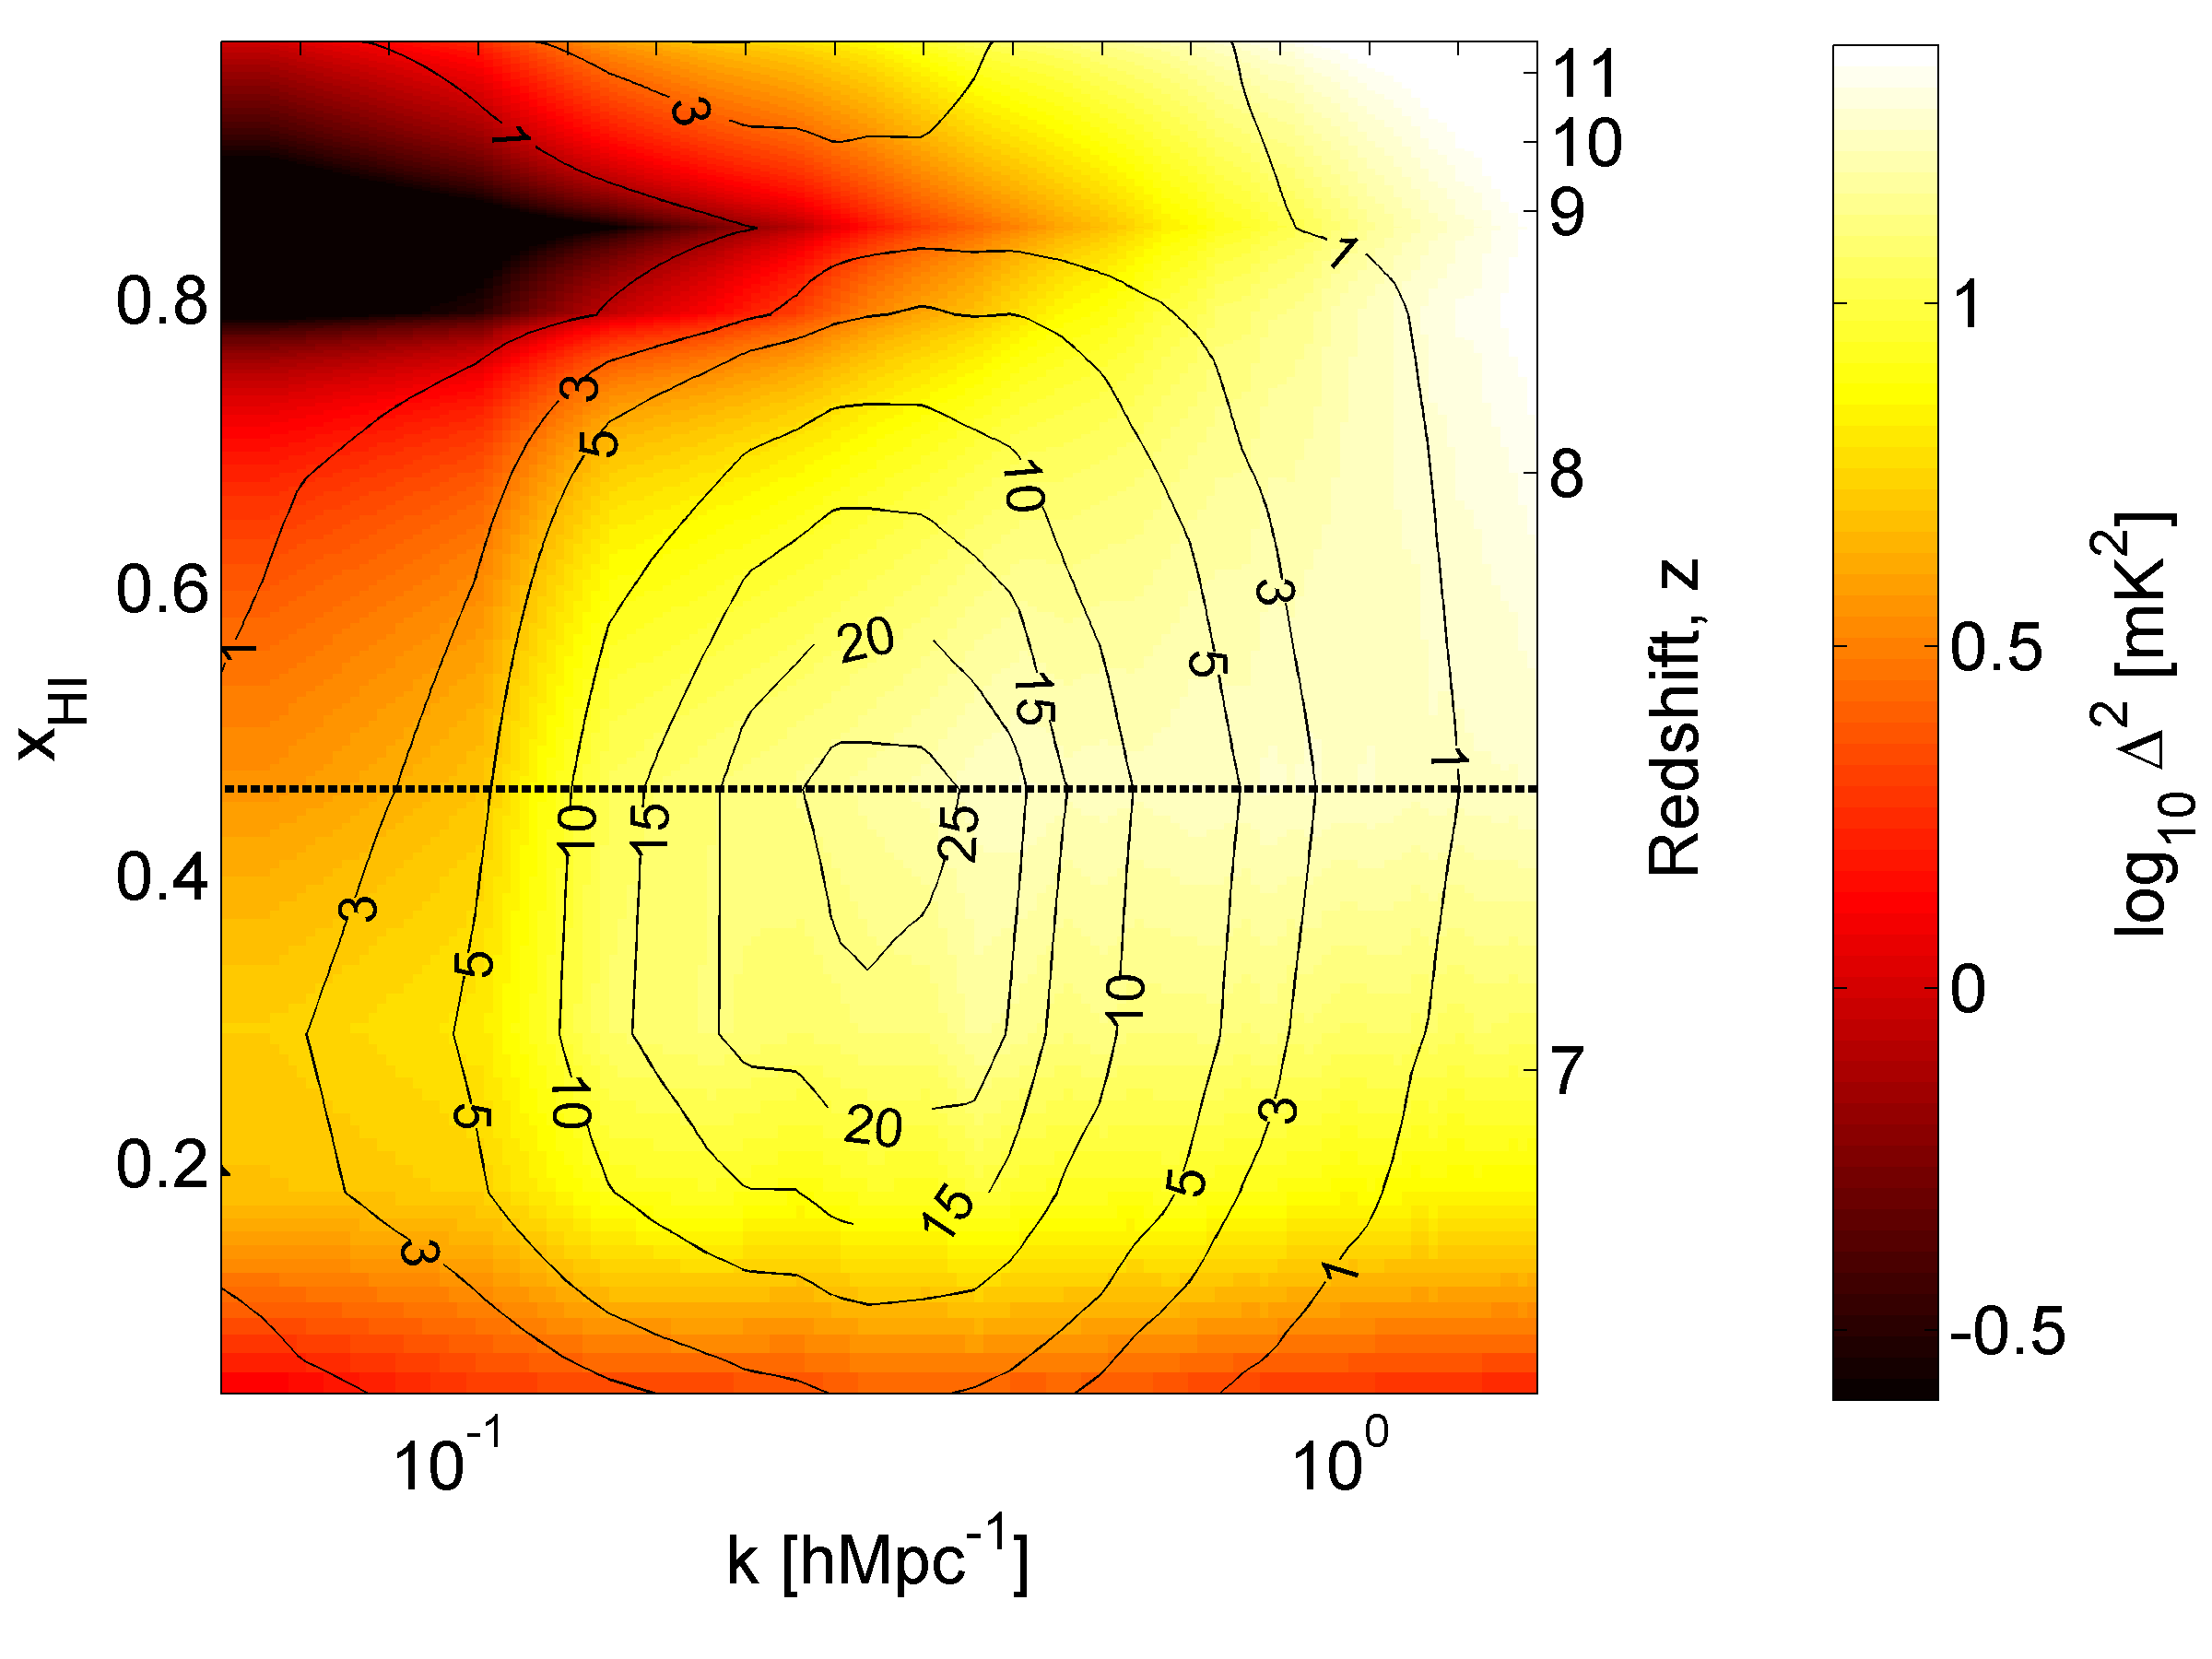
\includegraphics[height=2.25
in]{plots/hera_snr_contour.png} \caption{\small Left: Power-spectrum
sensitivities for three stages of HERA (solid) relative to a fiducial model
(dashed, with corresponding line in right panel), for 180-day drift-scan
observations toward the galactic pole, excluding modes that are expected to be
dominated by systematics.  In each stage, improvement in analysis software
expands the range of modes that are not systematics-dominated.  Right:
Simulations of 21~cm power spectrum amplitudes (color scale;
\citealt{lidz_et_al2008}) as a function of neutral fraction, $x_{\rm HI}(z)$,
with contours indicating the predicted detection significance with HERA-568.
%The spectrum initially follows the dark matter fluctuations at the upper edge
%of the plot, falls as the densest regions reionize at $x_i=0.8$ (inside-out in
%this model), rises and flattens as galaxies ionize large bubbles in the IGM
%($x_i$ 0.6--0.2, $x_i=0.5$ corresponds to the line in the lefthand panel),
%before falling again as reionization completes at the bottom of the plot.
}\label{fig:eor_pspec} \end{figure}
% XXX from carilli:
%3. fig 2b:  dotted line at z=7.5 should be dash to match format in 2a. also,
%caption should include some statement about degeneracy in x-z 


%\begin{figure}[!ht]\centering
%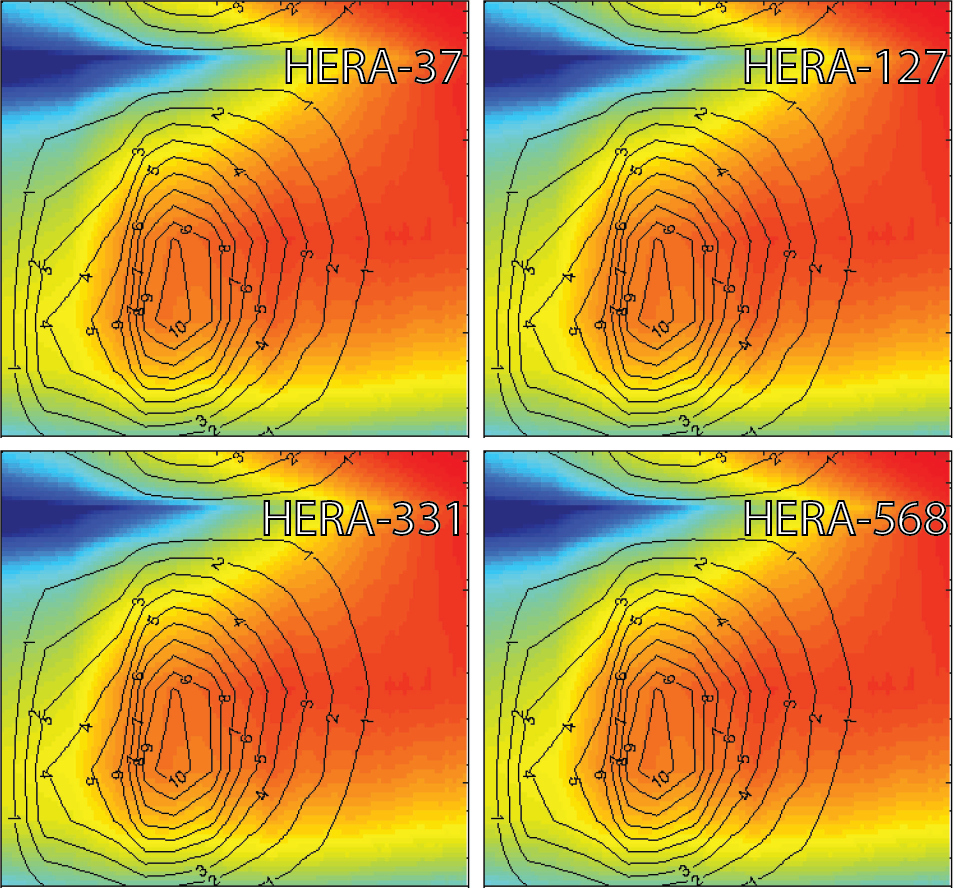
\includegraphics[width=4in]{plots/FourPanContour.png}
%\caption{\small
%[XXX: Replace with a plot that has the proper axes and color %bar.  Make some statement
%about detection at the earliest stages as well as the potential to do more.
%}\label{fig:FourPanContour}
%\end{figure}

\vspace{-0.25in}
\section{Foregrounds \& Lessons Learned from PAPER and MWA}
\label{LessonsSec}

The challenge of 21~cm cosmology is isolating the faint EoR signal from
astrophysical foregrounds that are 4--5 orders-of-magnitude brighter, as seen
in the lefthand panel of Figure \ref{fig:twoFGViews}. The major breakthrough in
21~cm cosmology---what enables us to propose HERA now---is the discovery of the
EoR Window.

21~cm cosmology observations and foreground isolation are best understood in
the three dimensional wavenumber space $\k$.  Because the \HI emission is a
narrow spectral line, the observed frequency of the emission can be mapped to
redshift or line-of-sight distance to provide an observed volume $\{x,y,z\}$ in
cMpc. This observed volume is Fourier transformed into a three dimensional
wavenumber cube $\{k_{x}, k_{y}, k_{z}\}$. For graphical simplicity the angular
wavenumbers are typically averaged ($\{k_{x},k_{y}\}\rightarrow\kperp$) to
produce line-of-sight wavenumber $\kpar$ vs.\ angular $\kperp$ figures. 
%Interferometric measurements are of the angular Fourier modes in many
%frequency channels (visibilities), so in the absence of widefield effects only
%a Fourier transform in the frequency direction and a coordinate mapping is
%needed to obtain the 3D $\{k_{x}, k_{y}, k_{z}\}$ measurements
%\citep{morales_hewitt2004}.) 
Spatial isotropy allows measurements within the 3D wavenumber space to be
squared and averaged in shells to produce the spherical power spectrum
presented in Figure \ref{fig:eor_pspec}.

% XXX carilli wants recombination lines out of this paragraph
The astrophysical foreground emission is spectrally very smooth (synchrotron \&
Bremsstrahlung emission) or at known editable frequencies (radio recombination 
lines). The advance in 21~cm cosmology has been understanding how this
foreground emission interacts with the instrument to produce the EoR Window.
Through a concerted theoretical and observational campaign
\citep{morales_et_al2012,parsons_et_al2012b,vedantham_2012,Datta_2010,hazelton_et_al2013,pober_et_al2013,parsons_et_al2013,dillon_et_al2013b}
we now understand that the foreground contamination is confined to a `wedge' in
$\kpar$ vs.\ $\kperp$, as demonstrated by the PAPER observations in the
righthand panel of of Figure \ref{fig:twoFGViews}. This wedge is the result of
the smooth spectrum foregrounds (low $\kpar$) interacting with the inherent
chromaticity of an interferometer. This leaves the region above isolated from
the foreground emission---a window through which we can observe the EoR.
% XXX carilli: might add that this isolation requires an optimally designed experiment as we are doing for HERA

All observations have now confirmed the presence of the EoR Window
\citep{pober_et_al2013,dillon_et_al2013b}, including suppression by more than 3
orders-of-magnitude (6 in mK$^{2}$ units) to the thermal noise floor of current
PAPER observations \citep{parsons_et_al2013}. This is a major advance---we can
suppress foregrounds and we understand the instrumental and analysis
characteristics needed to perform the EoR measurement. The MWA and PAPER teams
have been at the forefront of developing the EoR Window, writing all of the
papers in the literature and developing the individual baseline
(delay-spectrum) and full power spectrum (imaging) analyses to exploit this
insight. 



\begin{figure}[t] \centering
%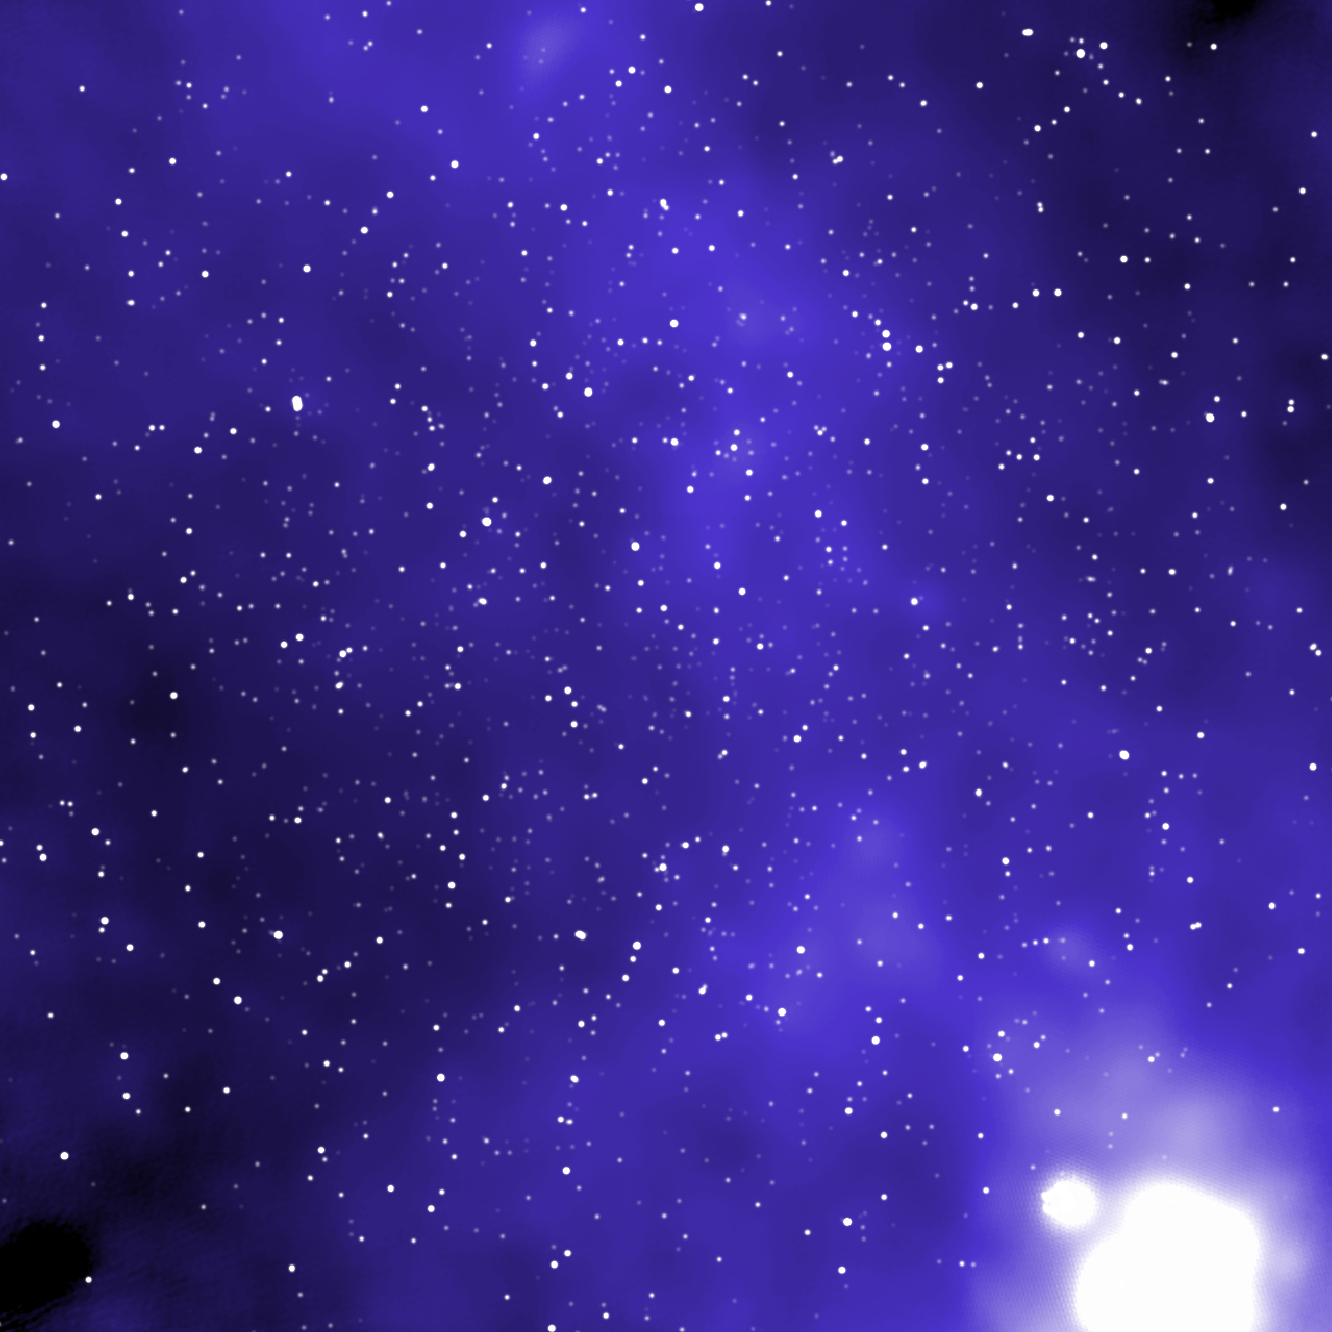
\includegraphics[width=6.5in]{plots/MWApretty.png} 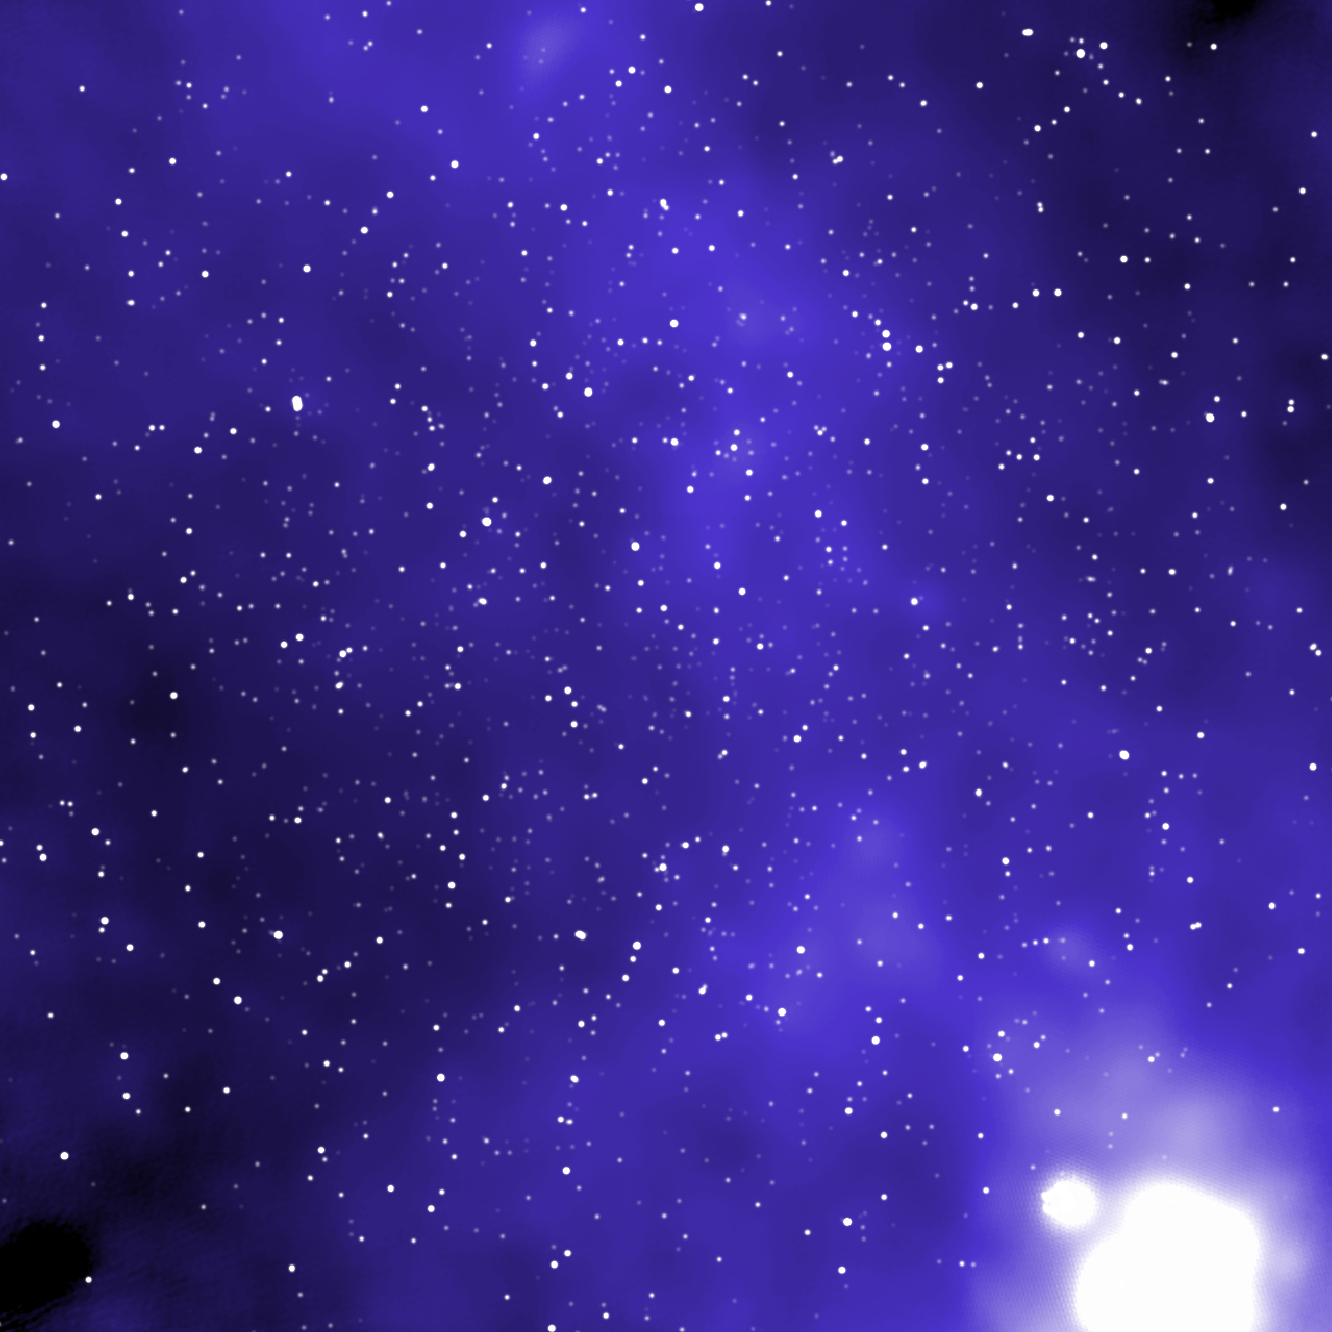
\includegraphics[width=3.6
%in]{plots/MWApretty.png}
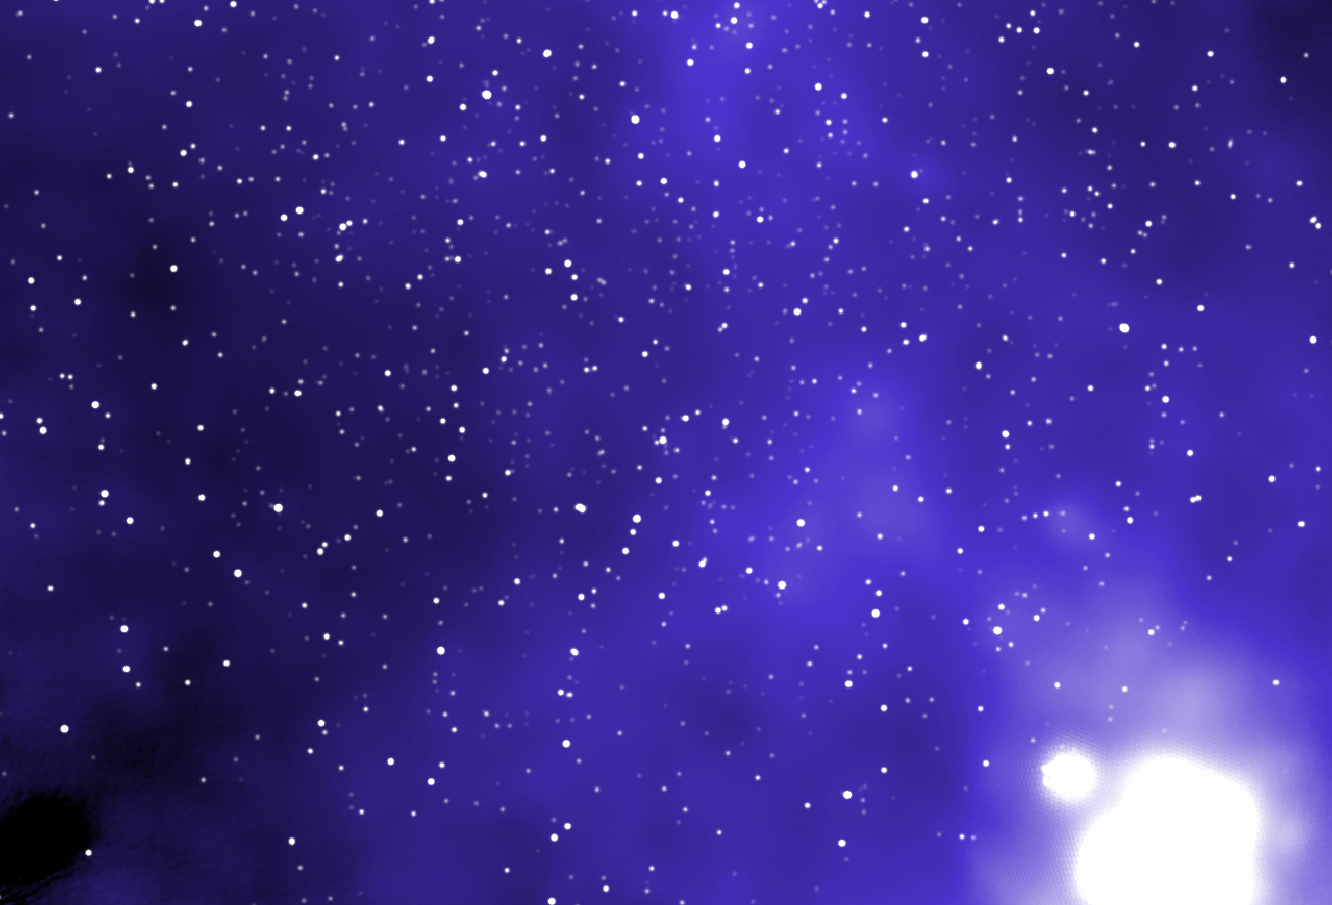
\includegraphics[height=2.5in]{plots/MWApretty_crop.png} ~ %gutter btwn
graphics
%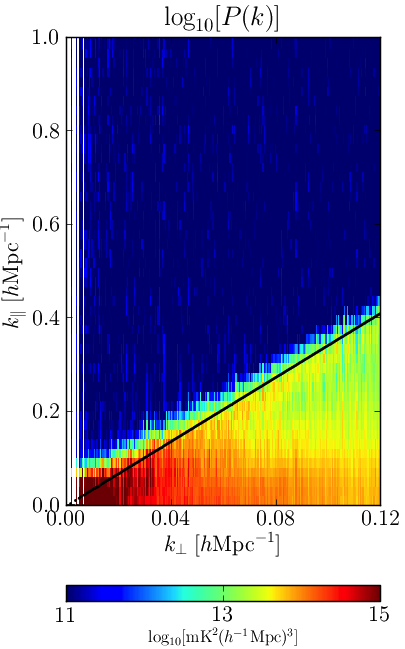
\includegraphics[width=2.4 in]{plots/wedge_tall.png}
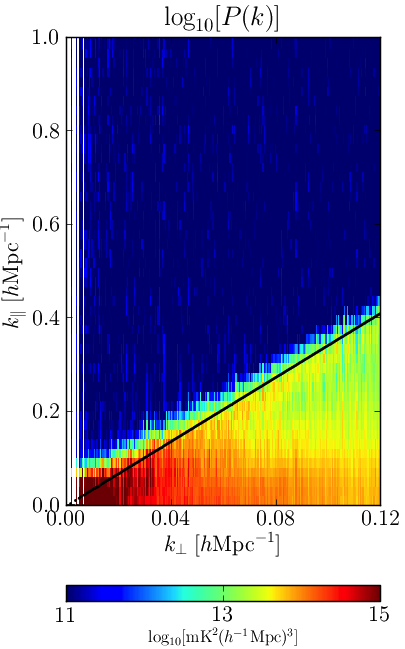
\includegraphics[height=2.5in]{plots/wedge_tall.png} \caption{\small Left:
Foregrounds imaged on the MWA using FHD software developed by Morales' group
\citep{sullivan_et_al2012}.  This image, which spans $\sim$$30^{\circ}$ and
includes both point-source and diffuse emission (e.g. the Vela and Puppis SNRs,
bottom-right), illustrates the power of imaging methods for reducing
polarization leakage and foreground systematics.  Right: Foreground systematics
become unsmooth (vertical axis) versus baseline length (horizontal).  The EoR
window (blue), predicted theoretically
\citep{morales_et_al2012,parsons_et_al2012b,vedantham_2012,Datta_2010}, and
verified empirically above \citep{pober_et_al2013}, is a region where
foreground systematics fall by orders-of-magnitude, leading to
sensitivity-limited upper limits and the first meaningful constraints on EoR
via 21~cm emission \citep{parsons_et_al2013}.
% XXX does the word "wedge" need to be mentioned?
}\label{fig:twoFGViews} \end{figure}
% XXX carilli: 8. fig 3: i think the MWA image is sort of too big relative to
% the wedge image. sort of dwarfs it.  also, the caption should state what the
% black line is in fig 3b.

%\begin{figure}\centering
%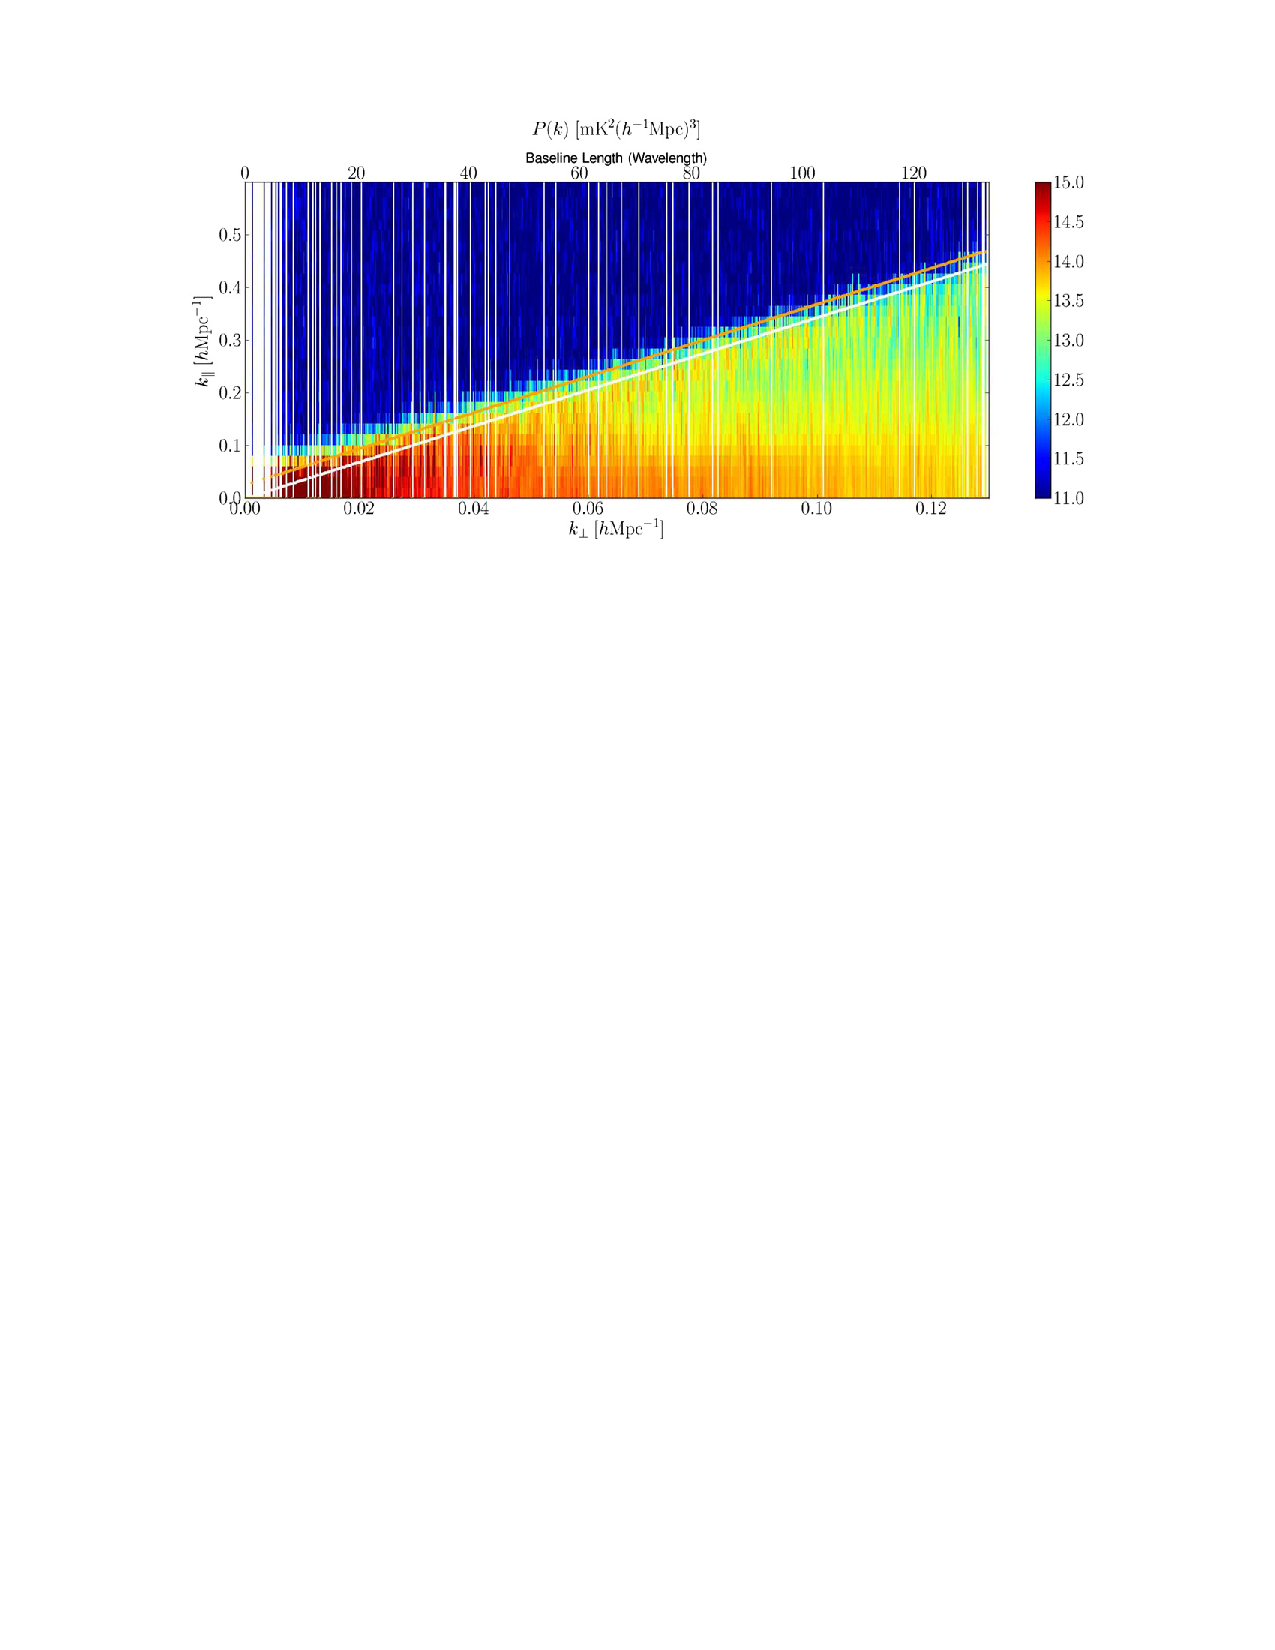
\includegraphics{plots/Pober_wedge.pdf}
%\caption{\small
%The EoR window as measured by PAPER.  Blue represents a region containing EoR signal but no foreground contamination.
%}\label{fig:EoRwindow}
%\end{figure}

%\begin{figure}[!ht]\centering
%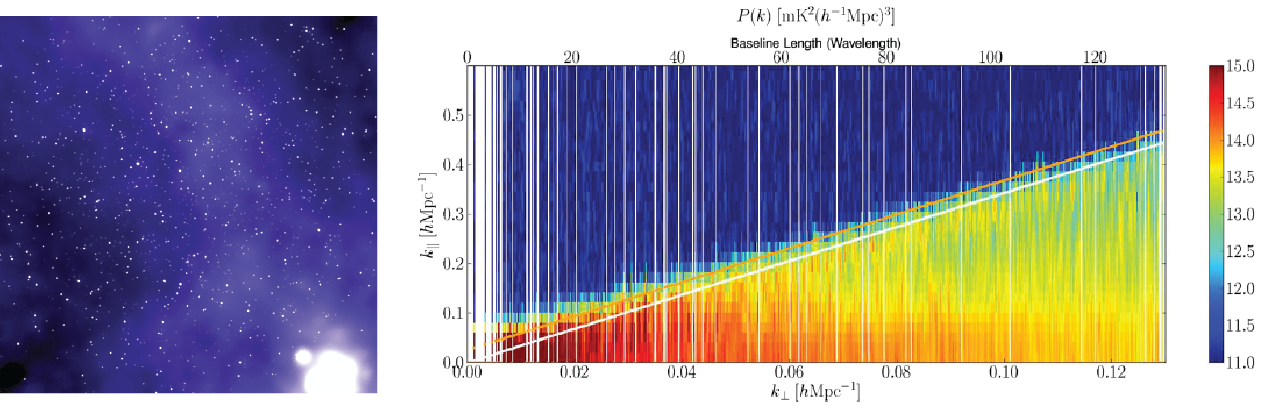
\includegraphics[width=1.0\textwidth]{plots/twoFgViews.png}
%\caption{\small
%[XXX: Redo in a more attractive way.]
%Left: Foregrounds in the image domain, as observed by the MWA using the Fast Holographic Deconvolution software package developed at the University of Washington.  Right: Foregrounds in the Fourier domain, as observed by PAPER.  The EoR window is the blue region containing EoR signal but relatively little foreground contamination.  Current experiments have begun to set interesting power spectrum limits by working in the EoR window.  HERA will take full advantage of both views of the sky, using maps of smooth spectrum and polarized foregrounds to enlarge the EoR window.
%}\label{fig:twoFGViews}
%\end{figure}




\vspace{-0.25in}
\section{HERA}
\label{PDsec}
\begin{figure}[t]\centering
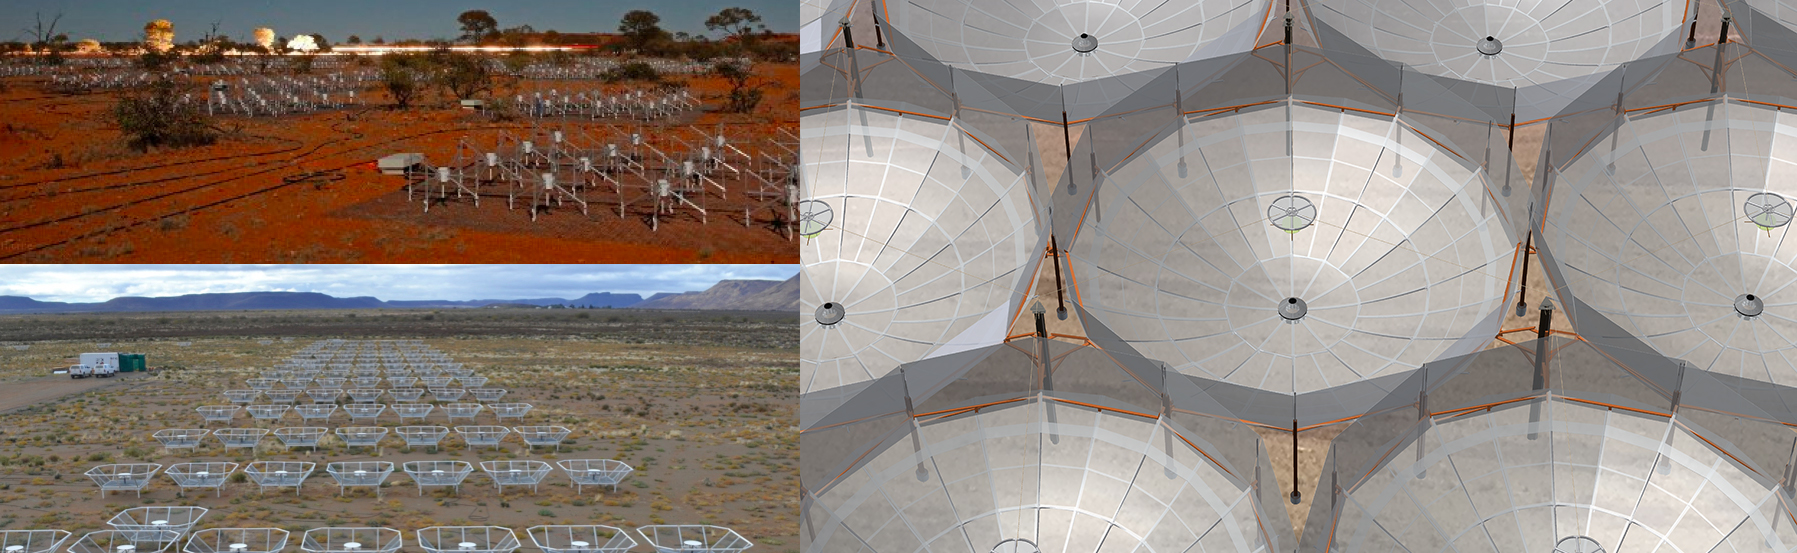
\includegraphics[height=2in]{plots/PAPER_and_MWA_and_HERA.jpg}
\caption{\small
Left: the MWA (top) and PAPER (bottom) arrays, each with 128 elements. Right:
the HERA element, which has been optimized for spectral smoothness and
stability. The core of HERA~568 consists of a redundant hexagonal array with
outrigger antennas (not shown) for imaging and foreground mitigation.
}
\label{HERAfig}
\end{figure}
%\begin{figure}[!ht]\centering
%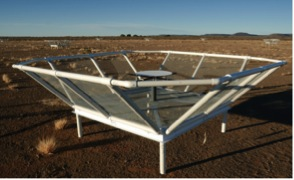
\includegraphics[height=1.75in]{plots/paper_element.jpg}
%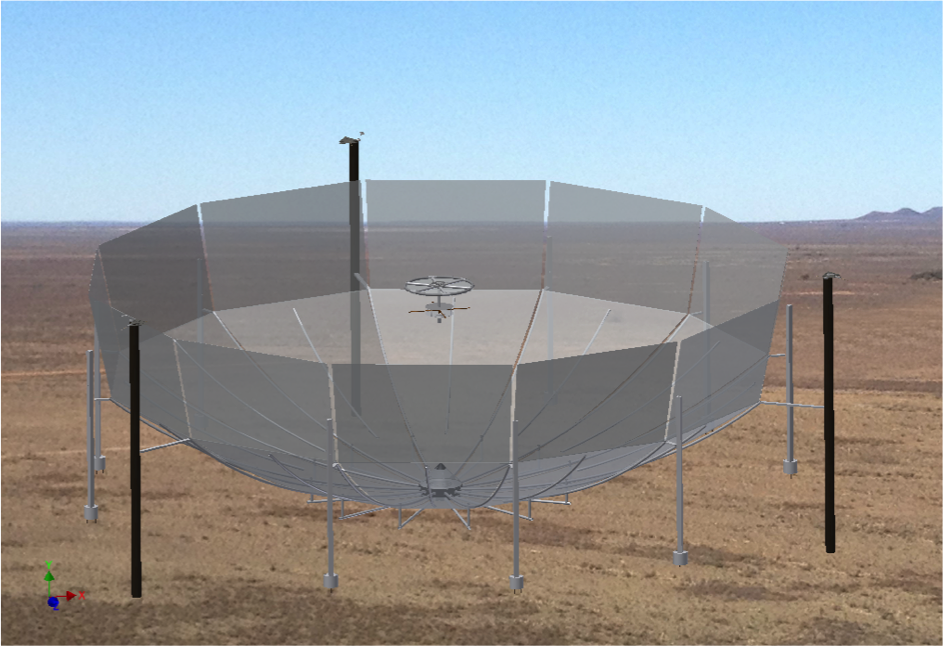
\includegraphics[height=1.75in]{plots/hera_dish.png}
%\caption{\small
%The PAPER element (left) provides a clean instrumental response as a function
%of frequency \citep{parsons_et_al2010,parsons_et_al2012b}, which is crucial to
%the foreground isolation shown in Figure \ref{fig:eor_pspec}.  A 14~m dish
%designed around the same feed (right) dramatically improves sensitivity while
%constraining the path length and amplitude of
%reflections to ensure that foreground isolation is not substantially degraded.  
%}\label{fig:hera_dish}
%\end{figure}

The HERA program entails a staged build-out to a 568-antenna array in South Africa that
incorporates the lessons learned from the first generation EoR observatories.
It features a 14~m zenith-pointing dish optimized for sensitivity and spectral
smoothness, a dense hexagonal core to enable redundant baseline calibration and
delay-spectrum analysis, and a distribution of outrigger antennas to provide
complete uv coverage to $\sim$700~m for foreground imaging and mitigation (see
Figure \ref{HERAfig}). HERA draws on the technical heritage of the MWA, PAPER,
EDGES and MITEoR. Specific examples include the antenna feed and correlator of
PAPER, receiver node and field digitization from the MWA, absolute radiometric
calibration from EDGES, redundant baseline calibration from MITEoR, the
delay-spectrum analysis from PAPER, and the precision imaging and foreground
removal software from the MWA.

%Incorporated into the design of HERA are new aspects that reflect our current understanding of the optimal balance between sensitivity and foreground systematics.  

The HERA antenna is an example of this technical heritage. The spectral
smoothness and the stability of the antenna response determine the precision to
which astrophysical foreground emission can be separated from the cosmological
21~cm emission. HERA uses the PAPER dipole feed---modified slightly for wider
bandwidth---suspended over a 14~m parabolic dish (Figure \ref{HERAfig}a). The
short ($\sim$5~m) focal height of the dishes is central to limiting the path
length of reflections whose time-delay gives rise to chromatic antenna
sensitivity. The zenith pointing enhances the stability of the antenna response
(PAPER), short cables to in-field digitizers limit the length of cable
reflections (MWA), and absolute calibration (EDGES) are all designed to provide
an extremely stable and smooth spectral response. Similarly the antenna layout
uses the dense core, outriggers, and symmetric configuration of the MWA,
combined with redundant baselines within the core (PAPER, MITEoR). Together
these advances enable HERA to have the science reach envisioned in the decadal
survey while fitting within the MSIP funding envelope.


HERA follows a staged build-out plan.  In
each deployment stage improvements are incorporated into the system and new
science capabilities are unlocked.  This approach has the advantage of
providing early access to science and reducing the project risk by testing systems
early and changing them incrementally.  As shown in Figure \ref{fig:eor_pspec}, each
stage of HERA brings an associated improvement in sensitivity that allows key
aspects of 21~cm reionization science to be addressed.  The timeline of HERA
development, along with the associated science products, is outlined below. 

\noindent{\bf Year 1--Infrastructure and First 37 Antennas (FY 2015)}.  
\begin{itemize}\setlength{\parskip}{0pt}\itemsep0pt
\vspace{-7pt}
  \item Install infrastructure $\sim$10~km from the current PAPER site at the Karoo Radio Observatory in South Africa. Includes ground leveling, power and basic network connectivity.
  \item Move existing PAPER-128 antennas, correlator, and EMC container to new site.
  \item Install first 37 HERA antennas and instrument with existing PAPER feeds and electronics. 
  \item Begin development of improved HERA baluns, receivers, feeds, and 
nodes using the PAPER and MWA technical heritage \citep{bradley_et_al2005,lonsdale_et_al2009,tingay_et_al2013} 
and the in-situ antenna calibration system based 
on EDGES \citep{rogers_2012}. Continue development of delay-spectrum \citep{parsons_et_al2012b}, 
Fast Holographic Deconvolution (FHD; \citealt{sullivan_et_al2012}) and 
optimal esitmator software \citep{dillon_et_al2013b}.
\end{itemize}


\noindent{\bf Year 2--Hardware Commissioning and Deep Foreground Survey (FY 2016)}.  
\begin{itemize}\setlength{\parskip}{0pt}\itemsep0pt
\vspace{-7pt}
  \item Commissioning observations using a hybrid array of 37 HERA antennas in a close-packed hexagon surrounded by 91 PAPER antennas in an imaging configuration.
  \item Perform a polarized foreground survey using hybrid-antenna capability of FHD. Determine on-sky beam response of HERA antennas to facilitate future source subtraction efforts.
  \item Finalize site infrastructure (high-bandwidth optical network, surveying, trenching).
  \item On-antenna commissioning of new feeds, receivers, nodes, and calibration systems in Green Bank and South Africa.
  \item Build out to 127 HERA antennas starts.
\end{itemize}


\noindent{\bf Year 3--HERA 127 and Detecting the Rise and Fall of Reionization (FY 2017)}.
\begin{itemize}\setlength{\parskip}{0pt}\itemsep0pt
\vspace{-7pt}
  \item Complete construction of HERA~127. Begin science observations Oct.\ 2016, again using the PAPER correlator.
  \item Begin analysis of a dataset capable of constraining the timing and duration of reionization. 
Analysis focuses on proven techniques based on PAPER delay-spectrum analysis, explorating subtraction of bright 
and polarized foregrounds.
  \item Begin deployment of HERA~331. Install node electronics for all 331 elements, and a new 331-element, 
GPU-based correlator in the Karoo Array Processing Building (KAPB).
  \item  Install new data storage infrastructure in the KAPB.  
Upgrade the UPenn analysis cluster.
\end{itemize}

\noindent{\bf Year 4--HERA 331 and Measuring the Evolution of the First Galaxies (FY 2018)}.
\begin{itemize}\setlength{\parskip}{0pt}\itemsep0pt
\vspace{-7pt}
  \item Finish construction of HERA~331. Begin science observations Oct. 2017.
  \item Complete science observations with HERA~331 Apr. 2018. Begin analysis of a dataset capable of
characterizing the evolution the power spectrum and determining properties of the first galaxies.
  \item Continue analysis software development, emphasizing imaging-based subtraction techniques for expanding the EoR window.
  \item Build out to 568 antennas begins, including outrigger antennas to facilitate imaging and better foreground removal.
  \item Complete pipelines for EoR processing of HERA~568.
\end{itemize}

\noindent{\bf Year 5--HERA 568, Imaging Reionization and Exploring the Dark Ages (FY 2019)}.
\begin{itemize}\setlength{\parskip}{0pt}\itemsep0pt
\vspace{-7pt}
  \item Finish construction of HERA~568. Begin science observations Oct. 2018.
  \item Analysis push to enable imaging of the largest structures and extracting the full sensitivity of 
the instrument, including partially coherent baselines. 
\end{itemize}


%\vspace{-0.25in}
%\subsection{The Transformative Science enabled by HERA}

% XXX Talk about specifically what science is being added in each stage of HERA
% XXX Bowman plot of constraints on ionization fraction versus redshift
% XXX new capabilities that are added in each stage
% XXX new low-frequency exploration, dark-ages plot from Aaron Ewall-Wice

\noindent
The staged buildout of HERA enables cutting edge science at each stage while
mitigating risk by allowing the team to learn from experience along the way.
HERA~127 will measure the rise and fall of the EoR power spectrum; HERA~331
will characterize the shape of the power spectrum and constrain the development
of the first galaxies; and HERA~568 will start to image reionization while
pushing power spectrum measurements into the Dark Ages.

% XXX check: was this stuff incorporated into a caption?
%In addition to pushing the sensitivity frontier, HERA will also extend the redshift frontier 
%to $z \sim 20$ and possibly beyond.  Measuring the power spectrum at higher, pre-reionization redshifts provides
%an incisive probe of astrophysical processes that are qualitatively different from those that
%drive reionization.  During the reionization era, the $21\,\textrm{cm}$ signal is driven by
%fluctuations in the ionization state of the IGM, while at higher redshifts the signal is determined
%by fluctuations in the spin temperature.  These fluctuations in turn depend sensitively on the nature of early heating sources  and their abundance, as well as on more exotic physics such as dark matter annihilation cross-sections.  Beginning with the midstages of its staged build-out, HERA will be in a unique position to probe the pre-reionization epoch that current-generation instruments are unable to reach (see Figure \ref{fig:x_i_Xray}).  With its ability to measure the power spectrum \emph{continuously} over an extremely large frequency range,
%HERA will also provide a longer lever arm for ionization history measurements than any other astronomical probe,
%as one can see in Figure \ref{fig:x_i_Xray}.
%
%{\sl Imaging reionization} In the later stages, HERA will become a powerful imaging instrument of cosmic reionization. Fiducial simulations of the expected \HI 21~cm signal on 25' scales predict regions with contrasts of about 10mK at 150MHz, or flux densities of up to 0.5 mJy/beam \citep{mcquinn_et_al2007}. The expected thermal noise for HERA 576 is 60 uJy, hence these regions could be detected at high confidence across redshifts $6<z<12$. Figure \ref{imaging} shows the predicted images of the \HI 21 structures  assuming the properties of HERA 547. The large scale structure is easily detected, and imaged, with the later stages of HERA. Of course, reaching these sensitivity levels relies critically on foreground synchrotron removal. We will be exploring foreground removal techniques throughout the program, and in particular, in the latter stages. The resulting \HI 21~cm images will provide a key reference for imaging of the large scale galaxy distribution (the sources of reionization), using CO or [CII] intensity mapping and/or nearIR surveys with WFIRST (see section ??).

% TBD: include in full prop? no space in science pre-proposal
%\begin{figure}
%\centering
%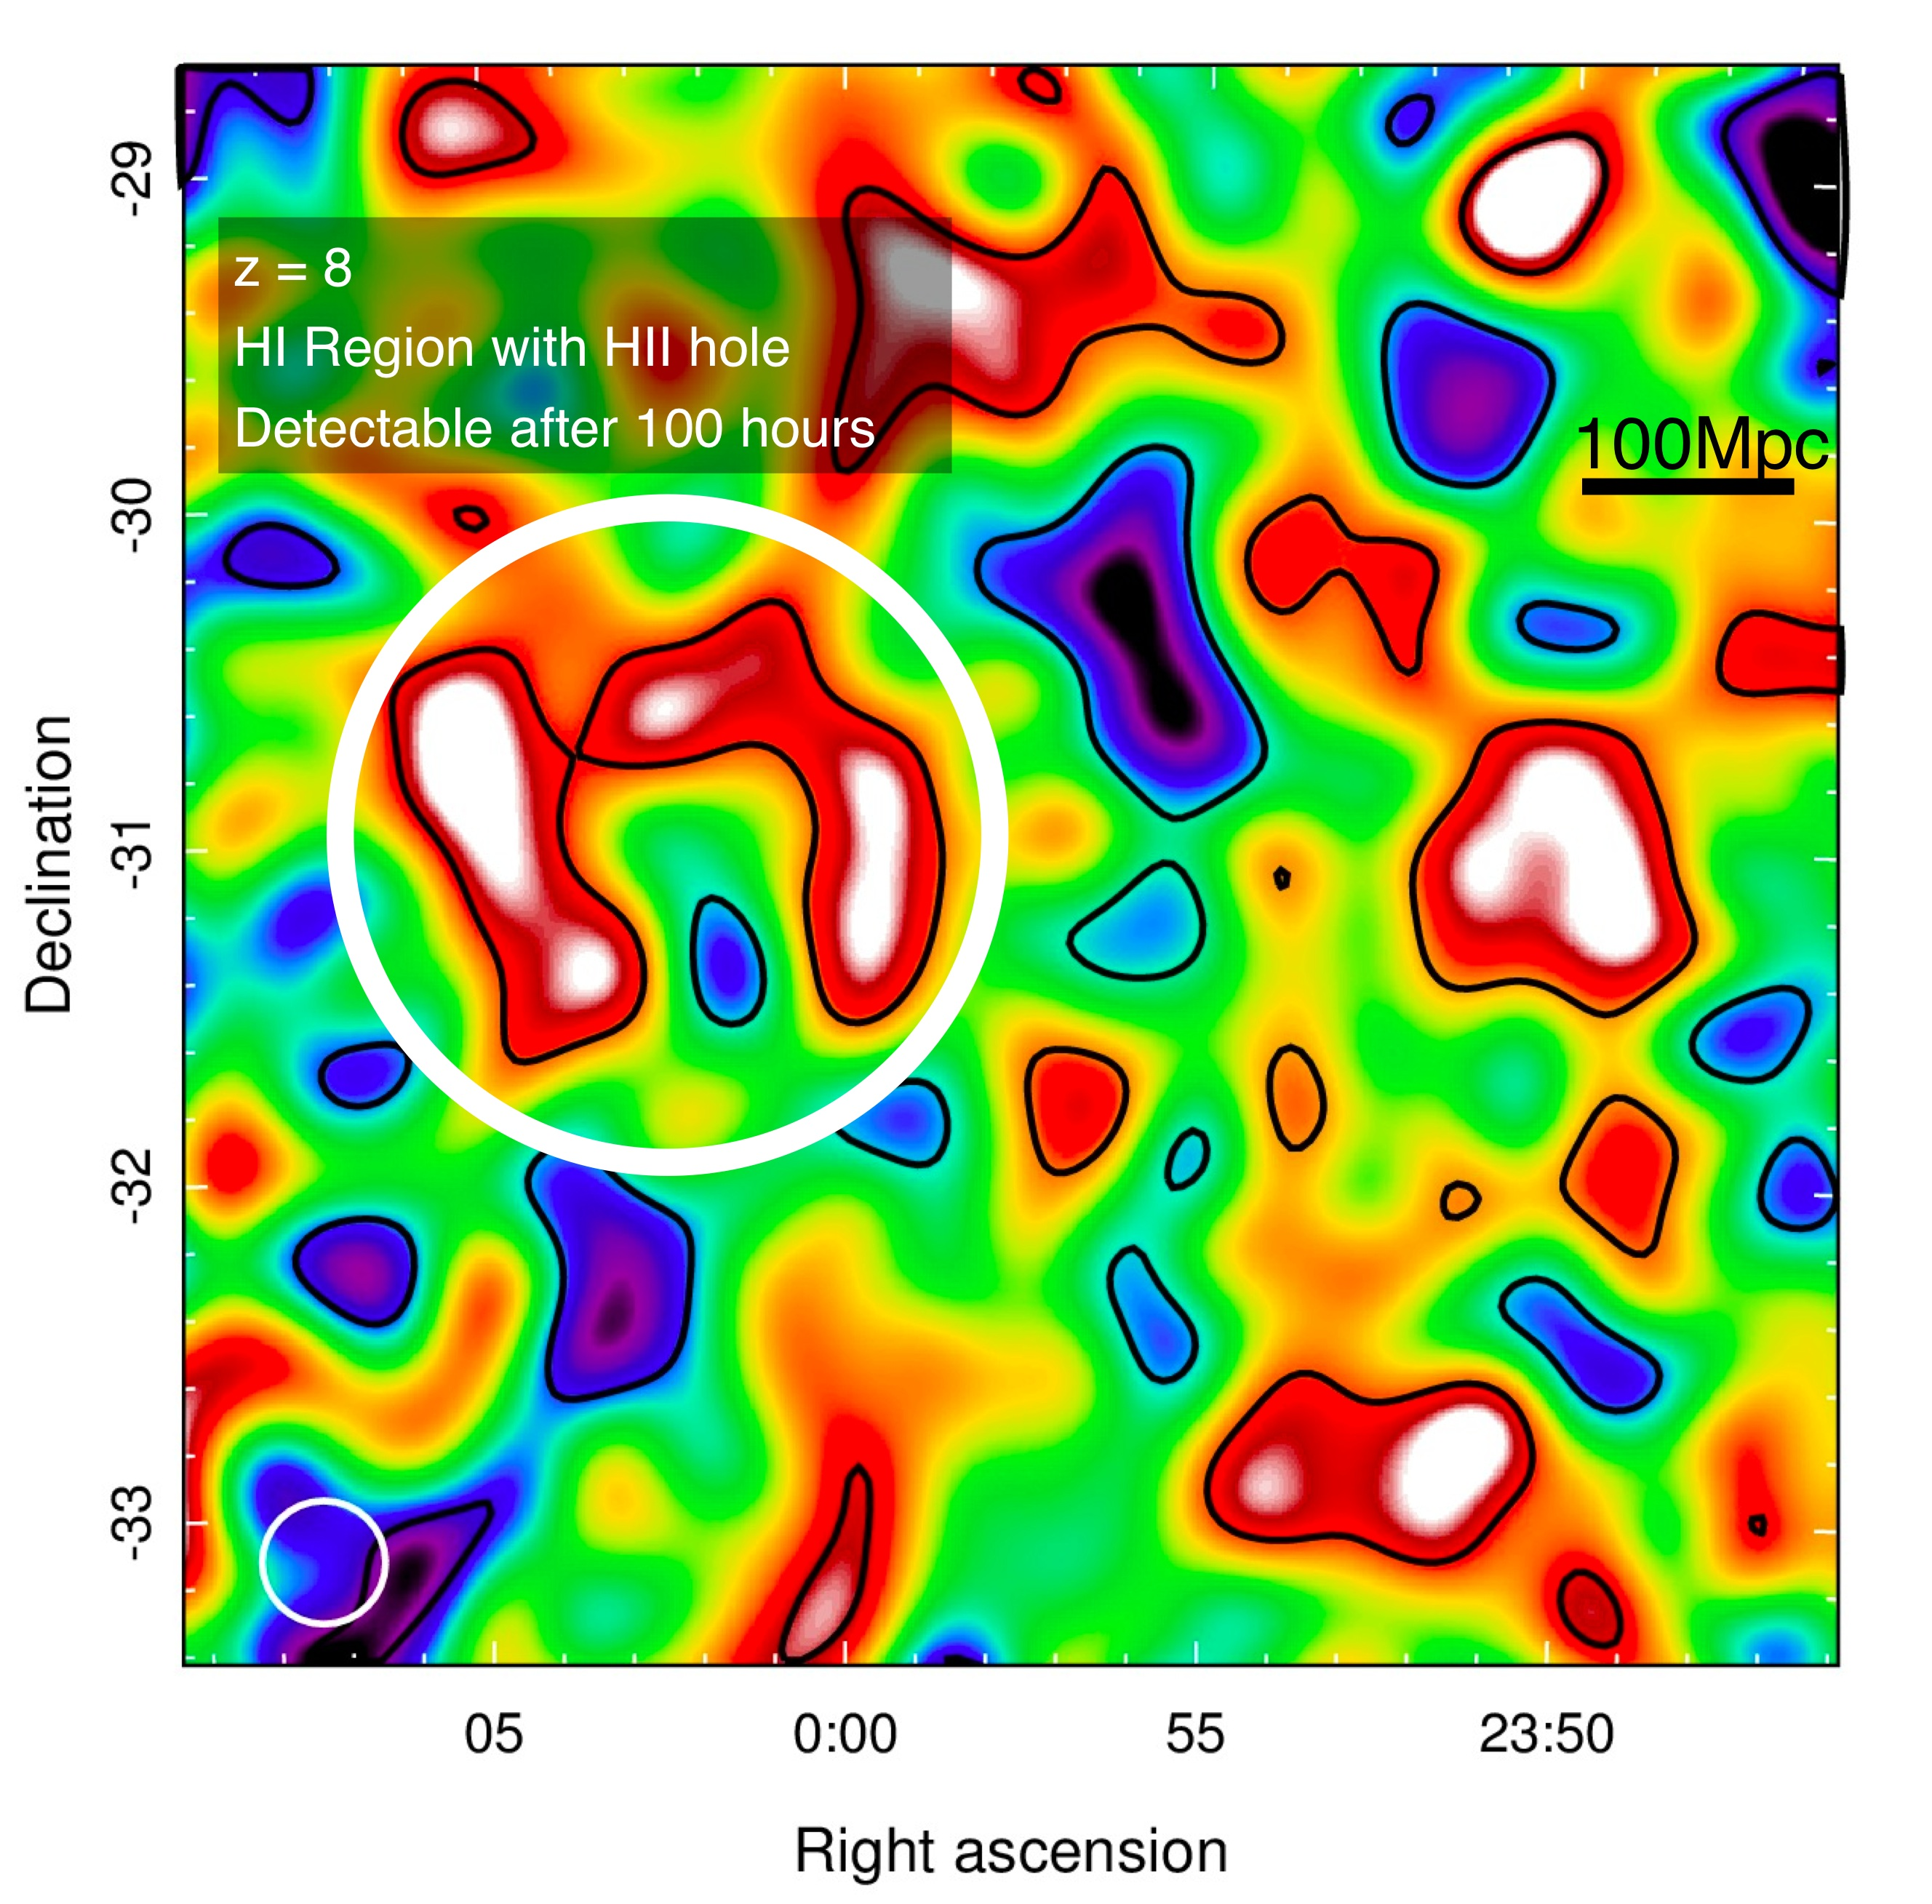
\includegraphics[height=4.in]{plots/HERA_z8_SNR_annotated_v2.jpg}
%\caption{\small With a surface brightness sensitivity, after filtering chromatic foregrounds, of 60uJy, the completed HERA array has enough sensitivity to detect regions of \HI and (in contrast) HII at SNR of 10 and above. Shown here is an instrumental simulation of observed \HI emission assuming 100 hours of observing. Large shells of \HI and deep HII regions are both detected at 10$\sigma$  \label{imaging}}
%\end{figure}


% XXX revert this section to pre-miguel edits
\vspace{-0.25in}
\section{Broader Impacts}
\label{BIsec}
\noindent {\bf Training Instrumentalists and Developing African Scientists.}
As a part of the HERA program we will train new instrumentalists and increase
the diversity of US graduate programs by preparing South African students for
admission to US degree programs.

The PAPER project has a history of employing South African undergraduate and
masters students as part of major deployment activities, and this work applies
directly to their academic program as field engineering experience.  We will
expand our South African outreach program during HERA, by recruiting talented
South African undergraduate and masters students for 3 month internships at the
HERA partner institutions. Each year one institution will host the SA cohort
(cohorts are more culturally appropriate than individual internships),
providing an REU-like experience focused on helping commission and operate
HERA. This experience will familiarize the students with the US graduate
schools, and give them the research experience and letters of recommendation
critical for future admission. 

%
%
%
%
%With scientific instruments coupled to the
%Moore's Law growth in the capabilities of digital electronics,
%new science opportunities are constantly arising, and existing
%facilities can fall rapidly into obsolescence.  To keep up,
%astronomy needs talented instrumentalists with a broad
%set of skills who can adapt to rapid changes in the field.
%%A sampling of the skills required includes the practical
%%application of antenna design, optics,
%%3D modeling, machining, circuit design, soldering, DSP algorithms, FPGA/GPU programming, network management,
%%computing systems, kernel optimization, interferometry, synthesis imaging, astrometry, statistical methods, linear
%%algebra, high-performance
%%computing, laboratory methods, and many, many others.  
%Some of these skills are taught
%in undergraduate and graduate
%curricula, but many are acquired through experience.  Moreover,
%many students who arrive at graduate school in astronomy and physics
%lack preparation in
%engineering, programming, and laboratory skills, and the students
%who have these skills 
%are often diverted to other field.
%
%This proposal addresses the loss of talented
%astronomers involved in instrumentation by
%targeting the gap in preparation between the
%undergraduate and graduate level of involvement in instrumentation.
%In addition to involving young graduate
%students at all institutions in the the developement, deployment,
%commssioning, and characterization of all stages of the HERA instrument,
%this proposal specifically funds a recurring specialist position
%position at UC Berkeley's RAL, offered each year to a
%person who gains practical experience working alongside professional RAL engineers
%on devloping the HERA instrument, with the goal of
%acquiring the skills required for
%pursuing graduate research in instrumentation.
%
%A second important activity of the HERA program, and
%one of the most personally fulfilling, is the cooperative education of
%minority students from South Africa in STEM fields. PAPER has an admirable history
%of employing technical and engineering undergraduate and masters
%students from 
%University of Kwazulu-Natal (UKZN) in Durban, as part of
%major engineering deployments. The work entails all
%aspects of telescope, receiver, correlator, and infrastructure construction and
%integration, and is incorporated into the UKNZ academic
%program as a key `practicum'. This
%student field engineering contribution has been fundamental for the
%success of PAPER.
%
%For HERA, we are expanding this cooperative student support beyond
%UKZN, and beyond technical internships. We have established formal collaborations
%with faculty at UCT, UWC, and UKZN to engage doctoral students from these
%institutions in all aspects of the project, from
%field engineering to rigorous data analysis. We plan to establish Ph.D.
%student exchanges, where students from ZA and USA make extended visits
%to HERA institutions in the partner nation.
%A goal of these efforts is to draw
%minority students from ZA into many of the graduate positions
%funded as part of the HERA project, and, though involvement in the
%program, to help ensure that these students are well positioned for
%success.

% TBD
%Notes:
%
%1. For the final proposal, we should get a supporting letter from 
%Durban and other Unviersities wrt student program. 
%
%2. I have read the 'Faculty Bridges' documents from Sheth at NRAO.
%Unfortunately, this program is just getting started, and it is not
%formally recognized by the NSF, nor funded. If this becomes more
%concrete over the next 4 months, we might consider adding a sentence
%that student exchanges will be facilitated by the formal agreements
%established by the 'Faculty Bridges' program.  However, for now, I
%have left this out.

\vspace{5 pt}
\noindent {\bf Public Data Products.}
On the HERA timescale a number of new observations will come on line that would
benefit from cross-comparison with the power spectra and images produced by
HERA. These include providing the reionization environment for JWST and ALMA
galaxy and cluster observations; cross-correlation with WFIRST near-IR surveys;
and cross-correlation with CMB polarization observations. The HERA measurements
will be released to the community after an 18~month proprietary period and
hosted at MIT. These data products will include foreground subtracted cubes for
cross-correlation, deep images of reionization from HERA~568, compressed
visibilities for re-analysis, snapshot continuum images for transient
observations, and wide-field maps from the survey made in the first two years.

% XXX are each of these in there?
%\item wide-field sky maps, made with 91 PAPER antennas in the first 2 years, 
%\item high-speed continuum images, generated as part of operational data analysis at MIT,
%\item deep, foreground-subtracted image products for use with other surveys and instruments,
%\item calibrated, compressed visibilities and the associated metadata database, upon request, and
%\item full-sensitivity data products from each stage of the HERA instrument, disseminated

% XXX include some of this above
%In parallel to the
%unique capabilities of the 21~cm line as a probe of neutral gas during
%reionization, powerful
%techniques are being explored to probe 
%the distribution of star forming galaxies and AGN droving reionization,
%and the ionized regions themselves.  
%CO and [CII] `intensity mapping' experiments \citep{carilli2011,lidz_et_al2011,gong_et_al2011}, 
%and wide-field
%near-IR galaxy surveys by WFIRST, are being designed to map the
%galaxy distributions during reionization.
%Follow-up high-resolution imaging of representative
%samples of these first galaxies with the JWST and ALMA will provide exquisite
%details of the distribution of the gas, dust, stars, and AGN inside the first
%galaxies. Likewise, there are signatures of large-scale structure in CMB images
%caused by streaming motions of ionized
%structures during reionization \citep{alvarez_et_al2006,tashiro_et_al2010}.
%
%Cross-correlating
%the 21~cm signal with these complementary views of reionization
%can potentially provide a complete imaging inventory of the sources and sinks of
%ionizing photons, and better constrain the physical processes involved in the
%formation of the first galaxies and AGN, and their influence on the neutral IGM
%(see \citealt{pritchard_loeb2012} for a review).  
%The cross correlation between 21~cm maps and very wide field galaxy distributions and the
%ionized gas distribution increases the reliability
%of each measurement,
%since foreground systematics are independent for the different
%techniques \citep{gong_et_al2011,alvarez_et_al2006,tashiro_et_al2010}. 
%The goal of imaging of
%reionization on 20' scales in year
%5 of HERA is well matched to the expected first results of intensity
%mapping experiments of large-scale structure in the galaxy distribution, as
%well as the final analysis of Planck CMB anisitropies. 
%We will work with teams from the complementary
%reionization studies to optimize the cross correlation analyses, thereby
%enhancing scientific return on all experiments. 
%
%Finally, MIT will host and 
%disseminate the following HERA data products:
%\begin{itemize}\setlength{\parskip}{0pt}\itemsep0pt
%\vspace{-7pt}
%\item wide-field sky maps, made with 91 PAPER antennas in the first 2 years, 
%\item high-speed continuum images, generated as part of operational data analysis at MIT,
%\item deep, foreground-subtracted image products for use with other surveys and instruments,
%\item calibrated, compressed visibilities and the associated metadata database, upon request, and
%\item full-sensitivity data products from each stage of the HERA instrument, disseminated
%within 2 years of observation.
%\end{itemize}

% TBD:
%following could be throw-away/repeditive: 
%
%The combination of imaging of the neutral IGM from the 21~cm experiments, with large scale galaxy distributions from CO/[CII] intensity mapping experiments and WFIRST surveys, and imaging of large scale ionized structures through CMB experiments, will map-out the full three dimensional structure of the Universe during reionization. In parallel, ALMA and JWST will probe the details of individual galaxies during reionization. Together, these programs will fulfill one of the primary Discovery objectives of NWNH, namely, exploring cosmic dawn and the epoch of first galaxy formation.
%
%1. A. Liu and M. Tegmark. PRD, 83:103006, 2011.
%2. C. L. Carilli, ApJ, 730:L30, 2011.
%3. A. Lidz et al. ApJ, 741:70, 2011.
%4. Y. Gong et al. ApJ, 728:L46, February 2011.
%5. http://www.ipac.caltech.edu/wfirst/overview/science/surveys/
%6. Alvarez et al. 2006, ApJ 647, 840
%7. Tashiro et al. 2010, MNRAS 420, 2617
%
%
%notes:
%
%1. Maybe Steve F. can put in some more interesting detailed physical implications?
%
%2. James can fill-in some CMB pol cross correlation details
%
%2. perhaps include fig 18 from Pritchard and Loeb (from Lidz et al., I think), or maybe one of the cross correlation PS analyses?

\vspace{-0.25in}
\section{Project Management Plan}
\label{PMPsec}

This project balances the light-weight management structure of PAPER/MWA
activities and the more formal structure required for larger-scale projects.
Construction management is centered at UC Berkeley's Radio Astronomy Laboratory
(RAL), headed by Aaron Parsons as the Project Director and DeBoer as
Project Manager. They will be assisted by Bob Goeke at MIT as a part-time
Project Engineer with a particular emphasis on interfacing with the NE based
antenna contractor.  A Site Manager will split their time between South Africa
and Berkeley and manage the construction activities by local South African
contractors. A SKA-SA Liaison will coordinate HERA, Meerkat, and SKA site
activities (supported by SKA-SA). Governance will be provided by a Board made
of this proposal's senior investigators, and will be operate using
super-majority policies. 

The scientific capability of HERA and the data analysis and publication will be
overseen by the Science Panel, and chaired by Project Scientist, Bowman. These
positions will rotate as needed expertise changes, and are appointed by the
Board.  As with the MWA and PAPER, observing
will be performed remotely with occasional site support
and maintenance headed by the Site Manager.

%Building on PAPER's excellent track record
%and the resources of ,
%this proposal consolidates responsibility and management of HERA
%fabrication and construction activities at RAL. Parsons serves as
%Project Director/Scientist; DeBoer serves as Project Manager and design engineer.
%Executive
%(Aguirre, Bradley, Hewitt, Morales, Werthimer)
%and Scientific (Aguirre, Bowman, Carilli, Furlanetto, Hewitt, Morales, Tegmark) Advisory Boards advise Parsons.
%A Site Manager supervises and manages
%construction activities executed by local contractors at the South African
%site, and reports to DeBoer.  A SKA-SA Liaison (supported by SKA-SA)
%interacts with DeBoer, the Site Manager and the SKA-SA board to
%coordinate HERA, Meerkat, and SKA site activities.
%
%An external advisory board evaluates the baseline design
%based on existing components in a Preliminary Design Review in Year 1.
%A Critical Design Review in Year 2 evaluates the
%production design that incorporates improvements to the analog system
%and feeds (Bradley), the node and correlator (Werthimer), the data storage
%system (Aguirre), and analysis software (Morales).
%Subsystem fabrication (electronics, antenna sub-assemblies, antenna assembly)
%are contracted to industry partners in the US and South Africa.   Construction on site proceeds
%with 2-3 teams of local contractors and laborers, managed by the site manager.  Observing proceeds 
%autonomously without local observers; SKA-SA
%provides occasional site support as necessary.

% XXX can we say this:
The estimated inherent contingency is $\sim$15\%, anticipating that project 
risk and contingency are handled by reducing
build-out with associated de-scoping of science capabilities.
% XXX add this?
%A baseline design using
%existing hardware establishes a low-risk path to core functionality and science.  Improved functionality
%results from successful development activities or is otherwise de-scoped.


\section{Why Now? Why Us?} % XXX better header?

This HERA proposal follows the vision for 21~cm observations laid out in NWNH.
PAPER and the MWA have already succeeded in the primary task envisioned in
NWNH---characterizing the astrophysical foregrounds and developing the hardware
and analysis advances needed to suppress the contamination. The discovery and
characterization of the EoR Window and the development of precision foreground
mitigation techniques have shown that foregrounds can be suppressed to the
thermal noise (\S \ref{LessonsSec}; \citealt{parsons_et_al2013}). While the MWA
and PAPER are pushing hard to detect the EoR PS, budget constraints have
dictated that a marginal detection is the best these instruments can achieve.
HERA will both ensure a high significance detection of the HI 21cm signal, as
well as provide powerful constraints on the rise and fall of reionization, how
early stars and structure formed, and physical processes at the end of the
cosmic dark ages (Figures \ref{fig:x_i_Xray} \& \ref{fig:eor_pspec}).

As envisioned in NWNH, the US EoR projects (PAPER, MWA, EDGES, MITEoR) have
pooled their expertise to develop the second generation HERA observatory. This
has created a small collaborative team with a deep well of scientific
experience---the majority of papers on EoR observations are authored by members
of the HERA team. By leveraging this expertise the HERA design is significantly
less expensive than envisioned in NWNH, while having greater scientific reach.

The last few years have been very productive for the EoR community---we
understand the foreground contamination and we are pushing the current
instruments to their thermal limits. We are now ready to build the HERA
instrument envisioned in NWNH and capitalize on the scientific promise of 21~cm
cosmology.


%\begin{table}
%\label{tab:params}
%\begin{tabular}{|l|rl|l|}
%\hline
%Parameter & Value & Units & Description \\
%\hline
%$N$  &  576  & & Number of Antennas \\
%$d$ & 14 & m & Antenna Diameter \\
%$f/d$ & 0.32 &  & Focal Length (fractional) \\
%$\Omega_{\rm P}$ & 0.026 & sr & Field of View (power) \\
%$\Omega_{\rm PP}$ & 0.013 & sr & Field of View (power$^2$) \\
%$\Omega_{\rm eff}$ & 0.052 & sr & Field of View (sensitivity) \\
%$B_{\rm samp}$ & 0--250 & MHz & Sampled Frequency Range \\
%$B_{\rm corr}$ & 100 & MHz & Correlated Bandwidth \\
%Config.    & 24 $\times$ 24 & & Square Grid Antenna Configuration\\
%$f/f_0$ & $1.5\cdot10^5$ & & Redundancy Metric (Parsons et al. 2012a) \\
%$A$ & 0.09 & km$^2$ & Total Collecting Area \\
%$\theta$ & 15 & arcmin & Angular Resolution (150 MHz) \\
%$b_{\rm max}$ & 500 & m & Maximum Baseline \\
%$T_{\rm sys}$ & 500 & K & System Temperature \\
%$t_{\rm obs}$ & 120 & days & Observing Time \\
%$t_{\rm day}$ & 6 & hrs & Observing Time Per Day\\
%$\Delta_{\rm N}^2$ & 1.6 & mK$^2$ & Expected Noise Level ($k=0.2 h\ {\rm Mpc}^{-1}$) \\
%SNR$_{21}$ & 11.7$\sigma$ &  & Expected Detection Significance (Lidz et al. 2008, $x_i=0.5$, 150 MHz) \\
%\hline
%\end{tabular}
%\end{table}

\clearpage
\setcounter{page}{1}
\thispagestyle{empty}
%\bibliographystyle{apj}
%\bibliographystyle{hapj}
\bibliographystyle{jponew}
%\bibliographystyle{unsrt}
\bibliography{biblio}


\end{document}

